\chapter{Clasa a XII-a}

\section{Primitive}

\begin{definitie}
$F$ este \textbf{primitivă} a lui $f$ pe intervalul $I$ dacă $F$ e derivabilă pe $I$ și $F'=f$. Mulțimea primitivelor este $\int f(x)\,dx=F(x)+\mathcal{C}$: două primitive diferă printr-o constantă \emph{pe interval} (consecința lui Lagrange).
\end{definitie}

\begin{teorema}[Existența]
Orice funcție \textbf{continuă} pe un interval admite primitive. Reciproc \textbf{nu}: există funcții discontinue cu primitive (ex. $f(x)=2x\sin\frac1x-\cos\frac1x$ pentru $x \neq 0$, $f(0)=0$, e discontinuă în $0$, dar are primitiva $F(x)=x^2\sin\frac1x$ pentru $x\neq0$, $F(0)=0$).
\end{teorema}

\begin{teorema}[Obstrucția Darboux]
Dacă $f$ admite primitive pe $I$, atunci $f$ are proprietatea lui Darboux pe $I$ (fiind derivata unei funcții --- Teorema Darboux din Partea I). Consecință practică: o funcție care \emph{nu} are Darboux (ex. cu o discontinuitate de speța I, sau cu $f(I)$ ne-interval) \textbf{nu admite primitive}. Acesta e testul standard la problemele „arătați că $f$ nu admite primitive''.
\end{teorema}

\begin{obs}
Atenție: Darboux e condiție \emph{necesară}, nu suficientă --- există funcții cu proprietatea Darboux fără primitive. La probleme de existență se folosesc frecvent: descompunerea $f=g+h$ cu $g$ continuă (are primitive) și analiza lui $h$; sau argumentul cu limita $\frac{F(x)-F(0)}{x}$ în puncte problematice.
\end{obs}

\begin{teorema}[Integrarea prin părți]
Dacă $f,g:I\to\mathbb{R}$ sunt derivabile cu derivatele continue, atunci $f'g$ și $fg'$ admit primitive pe $I$ și
\[
\int f(x)\,g'(x)\,dx=f(x)\,g(x)-\int f'(x)\,g(x)\,dx.
\]
\end{teorema}

\begin{teorema}[Prima schimbare de variabilă]
Fie $\varphi:I\to J$ derivabilă și $h:J\to\mathbb{R}$ cu primitive ($H$ una dintre ele). Atunci $(h\circ\varphi)\cdot\varphi'$ admite primitive pe $I$ și
\[
\int h\big(\varphi(x)\big)\,\varphi'(x)\,dx=H\big(\varphi(x)\big)+\mathcal C.
\]
Practic: fiecare linie din tabelul de mai jos are automat o „versiune compusă'' --- se înlocuiește $x$ cu $\varphi(x)$ și se cere factorul $\varphi'(x)$ sub integrală (de aceea nu mai listăm separat tabelul compus).
\end{teorema}

\begin{teorema}[A doua schimbare de variabilă]
Fie $\varphi:I\to J$ \textbf{bijectivă}, derivabilă, cu $\varphi'(x)\neq0$ pe $I$, și $f:J\to\mathbb{R}$. Dacă $h=(f\circ\varphi)\cdot\varphi'$ admite primitive pe $I$ (fie $H$ una), atunci $f$ admite primitive pe $J$ și
\[
\int f(x)\,dx=\big(H\circ\varphi^{-1}\big)(x)+\mathcal C.
\]
Deosebirea de prima: acolo recunoști în integrand tiparul $h(\varphi)\varphi'$ gata format; aici \emph{tu} introduci substituția $x=\varphi(t)$ și, la final, revii prin $\varphi^{-1}$ --- de aceea e nevoie de bijectivitate.
\end{teorema}


\medskip
\textbf{Exemplu.} $\displaystyle\int \frac{\cos x}{1+\sin^2 x}\,dx$.

Recunoaștem tiparul $h(\varphi)\cdot\varphi'$ cu $\varphi(x)=\sin x$ (deci $\varphi'(x)=\cos x$) și $h(t)=\dfrac{1}{1+t^2}$, a cărei primitivă e $H(t)=\mathrm{arctg}\,t$. Aplicând direct teorema:
\[
\int \frac{\cos x}{1+\sin^2 x}\,dx = \mathrm{arctg}(\sin x)+\mathcal C.
\]

\medskip
\textbf{Exemplu.} $\displaystyle\int \sqrt{1-x^2}\,dx$.

Lucrăm întâi pe $(-1,1)$. Introducem $x=\sin t$, $t\in\bigl(-\frac\pi2,\frac\pi2\bigr)$ (bijecție pe $(-1,1)$, cu $\varphi'(t)=\cos t>0$; în capetele $\pm\frac\pi2$ derivata s-ar anula, de aceea le excludem). Atunci $\sqrt{1-x^2}=\cos t$ și $dx=\cos t\,dt$:
\[
\int \sqrt{1-x^2}\,dx = \int \cos^2 t\,dt = \frac{t+\sin t\cos t}{2}+\mathcal C.
\]
Revenind prin $\varphi^{-1}$: $t=\arcsin x$, $\sin t=x$, $\cos t=\sqrt{1-x^2}$, deci
\[
\int \sqrt{1-x^2}\,dx = \frac{\arcsin x + x\sqrt{1-x^2}}{2}+\mathcal C.
\]
Formula rămâne valabilă pe tot $[-1,1]$: funcția din dreapta e continuă pe $[-1,1]$, iar derivata ei, $\sqrt{1-x^2}$, are limita $0$ în $\pm1$; prin corolarul teoremei lui Lagrange, e derivabilă și în capete, cu derivata $0=\sqrt{1-(\pm1)^2}$.

{Tabelul primitivelor uzuale (pe intervale pe care expresiile au sens)}
\[
\renewcommand{\arraystretch}{1.55}\setlength{\arraycolsep}{3pt}
\begin{array}{ll|ll}
\displaystyle\int x^{a}\,dx=\frac{x^{a+1}}{a+1}+\mathcal C\ (a\neq-1) &&
\displaystyle\int \frac{dx}{x}=\ln|x|+\mathcal C &\\[2pt]
\displaystyle\int a^{x}\,dx=\frac{a^{x}}{\ln a}+\mathcal C\ \ (e^x\mapsto e^x) &&
\displaystyle\int \frac{dx}{x^{2}+a^{2}}=\frac1a\,\mathrm{arctg}\,\frac xa+\mathcal C &\\[2pt]
\displaystyle\int \frac{dx}{x^{2}-a^{2}}=\frac{1}{2a}\ln\Big|\frac{x-a}{x+a}\Big|+\mathcal C &&
\displaystyle\int \frac{dx}{\sqrt{a^{2}-x^{2}}}=\arcsin\frac xa+\mathcal C &\\[2pt]
\displaystyle\int \frac{dx}{\sqrt{x^{2}\pm a^{2}}}=\ln\big|x+\sqrt{x^{2}\pm a^{2}}\big|+\mathcal C &&
\displaystyle\int \sin x\,dx=-\cos x+\mathcal C &\\[2pt]
\displaystyle\int \cos x\,dx=\sin x+\mathcal C &&
\displaystyle\int \frac{dx}{\cos^{2}x}=\mathrm{tg}\,x+\mathcal C &\\[2pt]
\displaystyle\int \frac{dx}{\sin^{2}x}=-\mathrm{ctg}\,x+\mathcal C &&
\displaystyle\int \mathrm{tg}\,x\,dx=-\ln|\cos x|+\mathcal C &\\[2pt]
\displaystyle\int \mathrm{ctg}\,x\,dx=\ln|\sin x|+\mathcal C &&
\displaystyle\int \mathrm{sh}\,x\,dx=\mathrm{ch}\,x+\mathcal C &\\[2pt]
\displaystyle\int \mathrm{ch}\,x\,dx=\mathrm{sh}\,x+\mathcal C && &
\end{array}
\]
Atenție la redactare: domeniul contează. De pildă, $\frac1x$ are primitiva $\ln x$ pe $(0,\infty)$ și $\ln(-x)$ pe $(-\infty,0)$, cu constante \emph{independente} pe cele două intervale (capcana „constantelor pe bucăți'' din secțiunea de redactare).


\begin{teorema}[Descompunerea în fracții simple]
Fracțiile raționale \textbf{simple} sunt: polinoamele, $\dfrac{A}{(x-a)^{n}}$ și $\dfrac{Bx+C}{(x^{2}+bx+c)^{n}}$ cu $b^{2}-4c<0$. Orice funcție rațională $\frac{P}{Q}$ se scrie \emph{unic} ca sumă finită de fracții simple: partea polinomială (câtul împărțirii, dacă $\deg P\ge\deg Q$) plus, pentru fiecare factor $(x-a)^{\alpha}$ al lui $Q$, termenii $\frac{A_1}{x-a}+\dots+\frac{A_\alpha}{(x-a)^{\alpha}}$, și pentru fiecare factor $(x^{2}+bx+c)^{\beta}$ ireductibil (adică $b^2-4c<0$: nu se descompune în factori de gradul întâi cu coeficienți reali), termenii $\frac{B_1x+C_1}{x^{2}+bx+c}+\dots+\frac{B_\beta x+C_\beta}{(x^{2}+bx+c)^{\beta}}$.
\end{teorema}

\begin{tehbox}{Rețeta de integrare a unei funcții raționale}
\begin{enumerate}[leftmargin=*, itemsep=1pt]
\item Dacă $\deg P\ge\deg Q$: împărțire cu rest --- partea polinomială se integrează direct.
\item Descompune în fracții simple (coeficienții: identificare sau valori particulare $x=a$).
\item $\displaystyle\int\frac{A\,dx}{(x-a)^{n}}$: direct din tabel (logaritm pentru $n=1$, putere pentru $n\ge2$).
\item $\displaystyle\int\frac{Bx+C}{x^{2}+bx+c}\,dx$: scrie numărătorul ca $\frac B2(2x+b)+\big(C-\frac{Bb}{2}\big)$ --- prima bucată dă $\frac B2\ln(x^{2}+bx+c)$ (derivata numitorului!), a doua, după forma canonică $\big(x+\frac b2\big)^{2}+\big(c-\frac{b^{2}}4\big)$, dă un $\mathrm{arctg}$.
\item Puterile $\ge2$ ale trinomului: recurență prin părți --- același mecanism ca în secțiunea de recurențe de integrale.
\end{enumerate}
\end{tehbox}

\subsection{Structura mulțimii funcțiilor cu primitive}

Notăm, pentru un interval nedegenerat $J$: $C(J)=$ funcțiile continue, $P(J)=$ funcțiile care admit primitive, $Da(J)=$ funcțiile cu proprietatea lui Darboux. Cele două teoreme de mai sus se rezumă într-o diagramă de reținut:
\[
C(J)\ \subsetneq\ P(J)\ \subsetneq\ Da(J),
\]
\textbf{ambele incluziuni fiind stricte}. Vizual:

\begin{center}
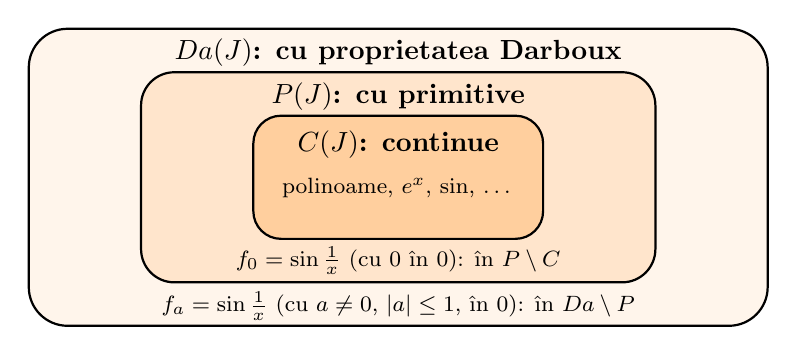
\begin{tikzpicture}[scale=0.92]
\draw[rounded corners=14pt, thick, fill=orange!8] (-5.1,-2.05) rectangle (5.1,2.05);
\draw[rounded corners=12pt, thick, fill=orange!20] (-3.55,-1.45) rectangle (3.55,1.45);
\draw[rounded corners=10pt, thick, fill=orange!38] (-2.0,-0.85) rectangle (2.0,0.85);
\node at (0,0.45) {\textbf{$C(J)$: continue}};
\node at (0,-0.15) {\footnotesize polinoame, $e^x$, $\sin$, \dots};
\node at (0,1.12) {\textbf{$P(J)$: cu primitive}};
\node at (0,1.72) {\textbf{$Da(J)$: cu proprietatea Darboux}};
\node at (0,-1.15) {\footnotesize $f_0=\sin\frac1x$ (cu $0$ în $0$): în $P\setminus C$};
\node at (0,-1.78) {\footnotesize $f_a=\sin\frac1x$ (cu $a\neq0$, $|a|\le1$, în $0$): în $Da\setminus P$};
\end{tikzpicture}
\end{center}

Martorii stricteții sunt amândoi din aceeași familie:

\begin{teorema}[Familia $\sin\frac1x$, clasificată complet]
Fie $a\in\mathbb{R}$ și $f_a:\mathbb{R}\to\mathbb{R}$, $f_a(x)=\sin\frac1x$ pentru $x\neq0$, $f_a(0)=a$. Atunci:
\[
f_a\ \text{admite primitive pe }\mathbb{R}\quad\Longleftrightarrow\quad a=0.
\]
În particular: $f_0\in P(\mathbb{R})\setminus C(\mathbb{R})$ (prima strictețe), iar $f_a$ cu $a\in[-1,1]$, $a\neq0$, are Darboux dar nu are primitive: $f_a\in Da(\mathbb{R})\setminus P(\mathbb{R})$ (a doua strictețe).
\end{teorema}
\begin{proof}
\emph{$a=0$ merge:} funcția $G(x)=x^2\cos\frac1x$, $G(0)=0$, e derivabilă peste tot, cu
\[
G'(x)=2x\cos\frac1x+\sin\frac1x\ \ (x\neq0),\qquad G'(0)=\lim_{x\to0}\frac{x^2\cos\frac1x}{x}=0.
\]
Deci $f_0(x)=G'(x)-2x\cos\frac1x$: diferență dintre o derivată și o funcție \emph{continuă} (prelungită cu $0$ în origine) --- ambele admit primitive, deci și $f_0$ (combinațiile liniare de funcții cu primitive au primitive).

\emph{$a\neq0$ nu merge:} prin absurd, dacă $f_a$ ar avea primitive, atunci $f_a-f_0$ ar avea primitive (diferență). Dar $f_a-f_0$ e funcția egală cu $a$ în $0$ și cu $0$ în rest --- imaginea ei e $\{0,a\}$, care nu e interval, deci nu are Darboux, deci nu are primitive. Contradicție.

\emph{Darboux pentru $a\in[-1,1]$:} pe orice interval care conține $0$, $f_a$ ia toate valorile din $[-1,1]$ (oscilația lui $\sin\frac1x$), deci imaginea oricărui interval e interval.
\end{proof}

\begin{obs}
Schema de demonstrație merită reținută ca metodă: (1) pentru a arăta că o funcție oscilantă \emph{are} primitive, o scrii ca $G'-(\text{ceva continuu})$ cu $G$ construit „cu un $x^2$ în față''; (2) pentru a arăta că \emph{nu} are, o compari prin diferență cu una care are --- spațiul $P(J)$ fiind închis la combinații liniare, obstrucția cade pe diferență, unde criteriile Darboux mușcă.
\end{obs}

\begin{teorema}[Produse de funcții cu primitive]
Produsul a două funcții cu primitive \textbf{nu} are, în general, primitive. Condiții suficiente ca $f\cdot g$ să admită primitive pe $J$:
\begin{enumerate}[leftmargin=*, itemsep=2pt]
\item $f$ admite primitive și $g$ e \textbf{derivabilă cu derivata continuă} ($g\in C^1$);
\item \emph{(Wilkosz)} $f$ admite primitive și e \textbf{mărginită} (superior sau inferior), iar $g$ e \textbf{continuă};
\item $f$ admite primitive și $g$ e derivabilă cu \textbf{derivata mărginită};
\item $f$ admite primitive, $f(x)\neq0$ pe $J$, iar $g$ e continuă.
\end{enumerate}
\end{teorema}
\begin{proof}[Demonstrația punctului 1 (și de ce 3 decurge din 2)]
Fie $F$ o primitivă a lui $f$. Din regula produsului, $(Fg)'=fg+Fg'$, deci
\[
f g=(Fg)'-F\,g'.
\]
Primul termen e o derivată (are primitive prin definiție); al doilea, $Fg'$, e \emph{continuu} ($F$ derivabilă deci continuă, $g'$ continuă), deci are primitive prin teorema de existență. Diferența are primitive. $\square$ \quad Pentru punctul 3, același truc reduce totul la primitivabilitatea lui $Fg'$: acum $g'$ e o derivată (deci are primitive) \emph{mărginită}, iar $F$ e continuă --- exact ipotezele lui Wilkosz cu rolurile $f\leftrightarrow g$ schimbate. Punctele 2 și 4 se citează ca atare.
\end{proof}

\textbf{Exemple rezolvate.} \emph{(a)} $h(x)=\ln(x^2+4)\cdot\sin\frac1x$ pentru $x\neq0$, $h(0)=0$, are primitive pe $\mathbb{R}$: ia $f=f_0$ (are primitive, prin teorema familiei; mărginită de $1$) și $g(x)=\ln(x^2+4)$ continuă --- Wilkosz. \emph{(b)} $h(x)=|x-a^2|\cdot\sin\frac1x$, $h(0)=0$: la fel, $g(x)=|x-a^2|$ e doar continuă (nu $C^1$ în $a^2$!), deci punctul 1 nu se aplică --- dar Wilkosz da. Acesta e și motivul pentru care Wilkosz merită știut: salvează exact cazurile cu $g$ continuă neneted.

\begin{teorema}[Câturi și compuneri, enunțuri]
\emph{(Jarník)} Dacă $f,g$ admit primitive pe $J$ și $g(x)\neq0$ pe $J$, atunci câtul $\frac fg$ are \textbf{proprietatea lui Darboux} pe $J$ --- dar poate să \emph{nu} admită primitive: pentru
\[
f(x)=8+\sin^3\tfrac1x,\quad g(x)=2+\sin\tfrac1x\ \ (x\neq0),\qquad f(0)=8,\ g(0)=2,
\]
ambele admit primitive pe $\mathbb{R}$, iar $\frac fg$ nu. \emph{(Compunerea)} Dacă $f:\mathbb{R}\to\mathbb{R}$ admite primitive, iar $g:J\to\mathbb{R}$ e de două ori derivabilă cu $g''$ continuă și $g'(x)\neq0$ pe $J$, atunci $f\circ g$ admite primitive pe $J$. (Motivul: dacă $F$ e o primitivă a lui $f$, atunci $f\circ g=(F\circ g)'\cdot\frac1{g'}$, iar $\frac1{g'}$ e de clasă $C^1$; se aplică punctul 1 al teoremei despre produse.) Exemplu-tip: dacă $f$ admite primitive pe $\mathbb{R}$, atunci și $x\mapsto f\big(x^3+x\big)$ admite, fiindcă $g(x)=x^3+x$ are $g'(x)=3x^2+1\neq0$ și $g''(x)=6x$ continuă.
\end{teorema}

\begin{obs}
Morala practică a întregii subsecțiuni: $P(J)$ e închis la sume și înmulțiri cu scalari, dar \textbf{nu} la produse, câturi sau compuneri --- fiecare operație cere o ipoteză suplimentară de regularitate pe unul dintre factori ($C^1$, mărginire, derivată mărginită). La problemele „arătați că $h$ admite primitive'' cu $h$ oscilant în jurul unui punct, drumul e aproape întotdeauna: desparte $h$ în (derivată explicită) $+$ (parte continuă), sau aplică Wilkosz cu factorizarea potrivită.
\end{obs}

\section{Integrala Riemann}

\begin{definitie}
Pentru o diviziune $\Delta: a=x_0<x_1<\dots<x_n=b$ cu norma $\|\Delta\|=\max(x_i-x_{i-1})$ și puncte intermediare $\xi_i\in[x_{i-1},x_i]$, suma Riemann este $\sigma_\Delta(f;\xi)=\sum_i f(\xi_i)(x_i-x_{i-1})$. Funcția $f$ este \textbf{integrabilă Riemann} pe $[a,b]$ dacă $\sigma_\Delta(f;\xi)$ tinde la un număr $\int_a^b f(x)\,dx$ când $\|\Delta\|\to 0$, indiferent de alegerea punctelor intermediare.
\end{definitie}

\begin{teorema}[Caracterizarea cu șiruri de diviziuni]
$f$ e integrabilă Riemann pe $[a,b]$ dacă și numai dacă pentru \emph{orice} șir de diviziuni $(\Delta_n)$ cu $\|\Delta_n\|\to0$ și orice alegeri de puncte intermediare $\xi^n$, șirul sumelor Riemann $\big(\sigma_{\Delta_n}(f;\xi^n)\big)$ converge; toate aceste limite coincid atunci cu $\int_a^b f$. Aceasta e versiunea „Heine'' a definiției --- și exact teorema care legitimează calculul limitelor de tipul $\frac1n\sum f\big(\frac kn\big)\to\int_0^1f$ din Partea a II-a: diviziunile echidistante sunt un șir particular cu norma $\frac1n\to0$.
\end{teorema}

\begin{teorema}[Proprietăți fundamentale]
Fie $f,g$ integrabile pe $[a,b]$ și $\lambda,\mu\in\mathbb{R}$. Atunci:
\begin{enumerate}[leftmargin=*, itemsep=1pt]
\item \textbf{Liniaritate:} $\lambda f+\mu g$ e integrabilă și $\int_a^b(\lambda f+\mu g)=\lambda\int_a^b f+\mu\int_a^b g$.
\item \textbf{Aditivitate (Chasles):} pentru $c\in(a,b)$, $\int_a^b f=\int_a^c f+\int_c^b f$; cu convențiile $\int_a^a f=0$ și $\int_b^a f=-\int_a^b f$, relația are loc pentru orice așezare a punctelor $a,b,c$.
\item \textbf{Monotonie:} dacă $f\le g$ pe $[a,b]$, atunci $\int_a^b f\le\int_a^b g$; în particular $\Big|\int_a^b f\Big|\le\int_a^b|f|\le(b-a)\sup|f|$ --- estimarea de bază a întregii teorii. Tot de aici: dacă $m\le f\le M$ pe $[a,b]$, atunci $m(b-a)\le\int_a^b f\le M(b-a)$.
\end{enumerate}
\end{teorema}

\begin{teorema}[Clase de funcții integrabile]
Sunt integrabile pe $[a,b]$: funcțiile continue; funcțiile monotone; funcțiile mărginite cu un număr finit de puncte de discontinuitate. Orice funcție integrabilă este mărginită. Modificarea lui $f$ într-un număr finit de puncte nu schimbă integrala.
\end{teorema}

\begin{teorema}[Criteriul lui Darboux]
Fie $f$ mărginită pe $[a,b]$. Pentru o diviziune $\Delta$, notăm cu $m_i,M_i$ infimumul și supremumul lui $f$ pe $[x_{i-1},x_i]$ și definim \textbf{sumele Darboux}
\[
\begin{aligned}
s(\Delta)&=\sum_i m_i\,(x_i-x_{i-1})\qquad\text{(inferioară)},\\
S(\Delta)&=\sum_i M_i\,(x_i-x_{i-1})\qquad\text{(superioară)},
\end{aligned}
\]
care încadrează orice sumă Riemann pe $\Delta$: $s(\Delta)\le\sigma_\Delta(f;\xi)\le S(\Delta)$. Atunci:
\[
f\ \text{integrabilă Riemann}\quad\Longleftrightarrow\quad
\forall\varepsilon>0\ \ \exists\,\Delta:\ \ S(\Delta)-s(\Delta)<\varepsilon.
\]
\end{teorema}

\begin{obs}[Cum se folosește criteriul]
Diferența $S(\Delta)-s(\Delta)=\sum_i(M_i-m_i)(x_i-x_{i-1})$ măsoară „oscilația totală'' a lui $f$ pe diviziune; criteriul spune că integrabilitatea $=$ oscilația poate fi făcută oricât de mică. Cele două clase mari ies în câte două rânduri:
\emph{monotonă} ($f$ crescătoare): $M_i-m_i=f(x_i)-f(x_{i-1})$, deci pentru diviziunea echidistantă cu pas $h$,
$S-s=h\sum_i\big(f(x_i)-f(x_{i-1})\big)=h\big(f(b)-f(a)\big)\to0$ (sumă telescopică!);
\emph{continuă}: prin teorema lui Cantor (Partea I), $f$ e \emph{uniform} continuă, deci pentru pas suficient de mic toate oscilațiile $M_i-m_i<\frac{\varepsilon}{b-a}$, și $S-s<\varepsilon$. Criteriul Darboux e, la olimpiadă, unealta standard pentru „arătați că $f$ e (sau nu e) integrabilă''.
\end{obs}

\begin{definitie}[Mulțime neglijabilă]
Intuiția: o mulțime $N\subset\mathbb{R}$ e „neglijabilă'' dacă poate fi \emph{ascunsă} sub o colecție de intervale a căror lungime totală e oricât de mică vrem. Formal: $N$ este \textbf{neglijabilă} dacă pentru orice $\varepsilon>0$ există intervale deschise $I_1,I_2,I_3,\dots$ (un șir, eventual finit) astfel încât
\[
N\subseteq I_1\cup I_2\cup I_3\cup\dots
\qquad\text{și}\qquad
\ell(I_1)+\ell(I_2)+\ell(I_3)+\dots<\varepsilon,
\]
unde $\ell(I)$ e lungimea intervalului $I$ (suma fiind o serie convergentă, dacă intervalele sunt o infinitate).

Să o simțim pe exemple, de la simplu la interesant:
\begin{enumerate}[leftmargin=*, itemsep=2pt]
\item \textbf{Un punct} $\{a\}$: îl acoperim cu $\big(a-\frac\varepsilon4,\,a+\frac\varepsilon4\big)$, de lungime $\frac\varepsilon2<\varepsilon$. Neglijabil.
\item \textbf{O mulțime finită} $\{a_1,\dots,a_k\}$: câte un interval de lungime $\frac{\varepsilon}{2k}$ în jurul fiecărui punct; lungime totală $\frac\varepsilon2<\varepsilon$. Neglijabilă.
\item \textbf{O mulțime numărabilă} $\{a_1,a_2,a_3,\dots\}$ (de pildă $\mathbb{Q}$!): aici e trucul frumos --- nu mai putem da tuturor aceeași lungime, dar putem da lungimi care \emph{scad geometric}: pe $a_n$ îl acoperim cu un interval de lungime $\dfrac{\varepsilon}{2^{n+1}}$. Lungimea totală:
\[
\sum_{n=1}^{\infty}\frac{\varepsilon}{2^{n+1}}=\frac{\varepsilon}{2}<\varepsilon.
\]
Deci \textbf{orice mulțime cel mult numărabilă e neglijabilă} --- inclusiv $\mathbb{Q}$, deși $\mathbb{Q}$ e densă în $\mathbb{R}$! Densitatea și „mărimea'' sunt lucruri diferite.
\item \textbf{Un interval $[a,b]$ cu $a<b$ NU e neglijabil:} orice acoperire a lui cu intervale are lungimea totală cel puțin $b-a$ (intuitiv clar; riguros, e o formă a lemei din Partea I despre intervale și mulțimi numărabile). Deci neglijabil înseamnă, la propriu, „fără grosime''.
\end{enumerate}
Reguli de calcul (toate cu aceleași idei): orice \emph{submulțime} a unei mulțimi neglijabile e neglijabilă (aceeași acoperire merge); o \emph{reuniune numărabilă} de mulțimi neglijabile e neglijabilă (acoperi mulțimea $A_n$ cu lungime totală $\frac{\varepsilon}{2^{n+1}}$ și aduni --- același truc geometric ca la exemplul 3).
\end{definitie}

\begin{teorema}[Criteriul lui Lebesgue, enunț]
Fie $f:[a,b]\to\mathbb{R}$ și $D$ mulțimea punctelor ei de discontinuitate. Atunci:
\[
f\ \text{integrabilă Riemann pe }[a,b]
\quad\Longleftrightarrow\quad
f\ \text{mărginită și}\ D\ \text{neglijabilă}.
\]
În cuvinte: poți fi discontinuu \emph{oriunde}, cu condiția ca locurile de discontinuitate, puse cap la cap, să nu aibă „grosime''.
\end{teorema}

\begin{obs}[Consecințe, citite prin exemplele de mai sus]
\begin{enumerate}[leftmargin=*, itemsep=2pt]
\item O funcție mărginită cu discontinuități \emph{finite sau numărabile} e integrabilă (exemplele 2--3). În particular, orice funcție \textbf{monotonă} e integrabilă --- discontinuitățile ei sunt numărabile, prin teorema din Partea I.
\item Funcția lui \textbf{Dirichlet} ($1$ pe $\mathbb{Q}$, $0$ în rest) \emph{nu} e integrabilă pe $[0,1]$: e discontinuă în \emph{orice} punct (ramurile nu se ating nicăieri --- corolarul lipirii, Partea I), deci $D=[0,1]$, un interval întreg --- exemplul 4, neneglijabil.
\item Funcția lui \textbf{Thomae}: $f\big(\frac pq\big)=\frac1q$ pentru fracții ireductibile, $f=0$ pe iraționale. Se arată că e discontinuă exact pe $\mathbb{Q}$ --- mulțime numărabilă, deci neglijabilă (exemplul 3): funcția \emph{este} integrabilă, cu $\int_0^1 f=0$. Contrast spectaculos cu Dirichlet: ambele „văd'' raționalele, dar Thomae le vede cu valori tot mai mici ($\frac1q\to0$), ceea ce o face continuă pe iraționale.
\end{enumerate}
Avertisment de redactare: demonstrația criteriului Lebesgue depășește liceul --- la concurs se citează ca atare sau se ocolește prin criteriul lui Darboux, care se demonstrează elementar.
\end{obs}

\begin{teorema}[Compunerea și integrabilitatea]
Dacă $g:[a,b]\to[c,d]$ e \textbf{integrabilă} și $\varphi:[c,d]\to\mathbb{R}$ e \textbf{continuă}, atunci $\varphi\circ g$ e integrabilă pe $[a,b]$.
\end{teorema}
\begin{proof}
Un rând, prin criteriul lui Lebesgue: în orice punct în care $g$ e continuă, $\varphi\circ g$ e continuă (compunere cu funcție continuă), deci $D_{\varphi\circ g}\subseteq D_g$; submulțimea unei mulțimi neglijabile e neglijabilă, iar $\varphi\circ g$ e mărginită ($\varphi$ continuă pe compact). 
\end{proof}

\begin{obs}[Compunerea a două integrabile NU e, în general, integrabilă]
Contraexemplul-bijuterie, cu două cunoștințe vechi ale fișei: fie $f$ funcția lui \textbf{Thomae} (integrabilă, prin consecința 3 de mai sus) și $g:[0,1]\to\mathbb{R}$, $g(0)=0$, $g(x)=1$ pentru $x\in(0,1]$ (integrabilă: o singură discontinuitate). Atunci
\[
(g\circ f)(x)=\begin{cases}1,& x\in\mathbb{Q}\cap(0,1],\\ 0,& x\in[0,1]\setminus\mathbb{Q}\text{ sau }x=0,\end{cases}
\]
adică, până la un punct, funcția lui \textbf{Dirichlet} --- neintegrabilă. Ordinea din teoremă e deci esențială: continuă $\circ$ integrabilă $=$ integrabilă, dar integrabilă $\circ$ integrabilă poate eșua; mai mult (subtil), chiar integrabilă $\circ$ \emph{continuă} poate eșua --- continuitatea trebuie să fie a funcției din \emph{exterior}.
\end{obs}

\begin{teorema}[Anularea integralei, foarte frecventă la ONM]
Dacă $f:[a,b]\to[0,\infty)$ este \textbf{continuă} și $\int_a^b f(x)\,dx=0$, atunci $f\equiv 0$. (Dacă $f(x_0)>0$, continuitatea dă $f>\frac{f(x_0)}2$ pe o vecinătate, deci integrala ar fi strict pozitivă.)
\end{teorema}

\begin{teorema}[Teorema fundamentală / Leibniz--Newton]
\begin{enumerate}[leftmargin=*, itemsep=1pt]
\item Dacă $f$ e continuă pe $[a,b]$, funcția $F(x)=\displaystyle\int_a^x f(t)\,dt$ este derivabilă și $F'=f$ (deci $F$ e primitiva care se anulează în $a$).
\item Dacă $f$ e integrabilă și admite primitiva $G$, atunci $\displaystyle\int_a^b f(x)\,dx=G(b)-G(a)$.
\item Cu capete variabile, pentru $f$ continuă și $u,v$ derivabile:
\[
\frac{d}{dx}\int_{u(x)}^{v(x)}f(t)\,dt=f\big(v(x)\big)\,v'(x)-f\big(u(x)\big)\,u'(x).
\]
\end{enumerate}
\end{teorema}

\begin{teorema}[Părți și schimbare de variabilă]
\begin{enumerate}[leftmargin=*, itemsep=2pt]
\item \textbf{Părți:} pentru $f,g$ derivabile cu derivatele continue pe $[a,b]$:
\[
\int_a^b f(x)\,g'(x)\,dx=\big[f(x)g(x)\big]_a^b-\int_a^b f'(x)\,g(x)\,dx.
\]
\item \textbf{Schimbarea de variabilă (I):} dacă $\varphi:[a,b]\to I$ e derivabilă cu derivata continuă și $f:I\to\mathbb{R}$ e continuă, atunci
\[
\int_a^b f\big(\varphi(x)\big)\,\varphi'(x)\,dx=\int_{\varphi(a)}^{\varphi(b)}f(t)\,dt
\]
--- \textbf{capetele se transformă odată cu variabila} (nu e nevoie ca $\varphi$ să fie monotonă: convențiile de semn din aditivitate acoperă și cazul $\varphi(a)>\varphi(b)$).
\item \textbf{Schimbarea de variabilă (II):} dacă $f$ e continuă pe $[a,b]$ și $\varphi:[c,d]\to[a,b]$ e bijectivă, derivabilă, cu derivata nenulă, atunci
\[
\int_a^b f(x)\,dx=\int_{\varphi^{-1}(a)}^{\varphi^{-1}(b)}f\big(\varphi(t)\big)\,\varphi'(t)\,dt.
\]
\end{enumerate}
Cea mai frecventă sursă de puncte pierdute la XII: uitarea transformării capetelor și verificarea superficială a ipotezelor lui $\varphi$ pe \emph{tot} intervalul (vezi capcanele din secțiunea de redactare).
\end{teorema}

\begin{teorema}[Prima formulă de medie]
Fie $f,g:[a,b]\to\mathbb{R}$ integrabile, cu $g\ge0$, și $m=\inf f$, $M=\sup f$. Atunci există $c\in[m,M]$ cu
\[
\int_a^b f(x)\,g(x)\,dx=c\int_a^b g(x)\,dx.
\]
Dacă, în plus, $f$ e \textbf{continuă}, constanta se realizează ca valoare: există $c\in[a,b]$ cu $\int_a^b fg=f(c)\int_a^b g$. Cazul $g\equiv1$: pentru $f$ integrabilă, $\int_a^b f=c\,(b-a)$ cu $c\in[m,M]$; pentru $f$ continuă, $\int_a^b f=f(c)(b-a)$.
\end{teorema}
\begin{proof}
Din $m\,g(x)\le f(x)g(x)\le M\,g(x)$ și monotonia integralei: $m\int g\le\int fg\le M\int g$. Dacă $\int g=0$, ambele capete sunt $0$ și orice $c$ merge; altfel, $c=\frac{\int fg}{\int g}\in[m,M]$. Pentru $f$ continuă, $[m,M]$ e exact mulțimea valorilor lui $f$ (Weierstrass $+$ Darboux, Partea I), deci $c=f(c')$ pentru un $c'\in[a,b]$.
\end{proof}

\begin{obs}[Interpretarea geometrică]
Pentru $f$ continuă și pozitivă: aria subgraficului pe $[a,b]$ coincide cu aria unui \emph{dreptunghi} de bază $b-a$ și înălțime $f(c)$ --- „nivelul mediu'' al funcției e atins efectiv. De reținut și limitarea: teorema garantează doar \emph{existența} lui $c$, nu unicitatea și nu vreo formulă pentru el.
\end{obs}

\begin{teorema}[Continuitatea integralei]
Fie $f$ integrabilă (nu neapărat continuă!) pe $[a,b]$, cu $|f|\le M$. Atunci $F(x)=\displaystyle\int_a^x f(t)\,dt$ este \textbf{lipschitziană}:
\[
|F(x)-F(y)|=\Big|\int_y^x f(t)\,dt\Big|\le M\,|x-y|,
\]
în particular continuă (chiar uniform). Așadar integrarea \emph{netezește}: din $f$ doar integrabilă iese $F$ continuă; din $f$ continuă iese $F$ derivabilă (Leibniz--Newton). Acest câștig de regularitate e motorul secțiunii despre ecuații funcționale rezolvate cu primitive.
\end{teorema}

\begin{teorema}[Teorema de medie a doua --- Bonnet]
Fie $f$ \textbf{monotonă} și $g$ continuă pe $[a,b]$. Atunci există $c\in[a,b]$ astfel încât
\[
\int_a^b f(x)\,g(x)\,dx\;=\;f(a)\int_a^{c}g(x)\,dx\;+\;f(b)\int_{c}^{b}g(x)\,dx.
\]
\end{teorema}
\begin{proof}[Demonstrație în cazul $f$ de clasă $C^1$]
Fie $G(x)=\int_a^x g(t)\,dt$, continuă, cu $G(a)=0$. Integrăm prin părți:
\[
\int_a^b fg=\int_a^b f\,G'=f(b)G(b)-\int_a^b f'(x)\,G(x)\,dx.
\]
Cum $f$ e monotonă, $f'$ păstrează semn constant; teorema de medie ponderată (cu ponderea $|f'|$) dă un $c\in[a,b]$ cu
$\int_a^b f'G=G(c)\int_a^b f'=G(c)\big(f(b)-f(a)\big)$. Atunci
\[
\int_a^b fg=f(b)G(b)-G(c)\big(f(b)-f(a)\big)=f(a)\,G(c)+f(b)\big(G(b)-G(c)\big),
\]
adică exact formula cerută. (Cazul general, $f$ doar monotonă, se obține prin sume Abel --- „integrarea prin părți discretă''; enunțul se citează ca atare.)
\end{proof}

\begin{obs}[La ce e bună a doua teoremă de medie]
La \emph{estimarea integralelor oscilante}: pentru $f$ monotonă pe $[a,b]$,
\[
\begin{aligned}
\Big|\int_a^b f(x)\sin(nx)\,dx\Big|
&=\Big|f(a)\int_a^c\sin(nx)\,dx+f(b)\int_c^b\sin(nx)\,dx\Big|\\
&\le\frac{2\big(|f(a)|+|f(b)|\big)}{n}\;\xrightarrow[n\to\infty]{}\;0,
\end{aligned}
\]
fiindcă orice primitivă a lui $\sin(nx)$ e mărginită de $\frac1n$ în variație. Este cazul „monoton'' al lemei Riemann--Lebesgue --- tip de problemă frecvent la ONM XII.
\end{obs}

\begin{obs}[Forma unilaterală a celei de-a doua formule]
Dacă $g$ e \textbf{descrescătoare și pozitivă} (iar $f$ integrabilă, de pildă continuă), formula se simplifică la un singur termen: există $\alpha\in[a,b]$ cu
\[
\int_a^b f(x)\,g(x)\,dx=g(a)\int_a^{\alpha}f(x)\,dx.
\]
(Se obține din forma cu două capete aplicată lui $g$ prelungit cu $g(b)\ge0$ „împins'' la $0$, sau direct prin sume Abel.) E forma cea mai comodă la estimări: dă imediat
$\big|\int_a^b fg\big|\le g(a)\cdot\max_{\alpha}\big|\int_a^{\alpha}f\big|$ --- toată oscilația lui $f$ e controlată de primitivele ei, iar $g$ contribuie doar cu valoarea din capătul „greu''.
\end{obs}

\begin{tehbox}{Simetrii și trucuri de calcul care apar constant la olimpiadă}
\begin{enumerate}[leftmargin=*, itemsep=1pt]
\item \textbf{Oglindirea:} $\displaystyle\int_a^b f(x)\,dx=\int_a^b f(a+b-x)\,dx$. Adunând cele două forme se elimină adesea partea „urâtă'' (clasic: $\int_0^{\pi/2}\frac{\sin x}{\sin x+\cos x}dx=\frac\pi4$; $\int_0^{\pi}xf(\sin x)dx=\frac{\pi}{2}\int_0^\pi f(\sin x)dx$).
\item \textbf{Paritate:} $f$ impară $\Rightarrow\int_{-a}^a f=0$; $f$ pară $\Rightarrow\int_{-a}^a f=2\int_0^a f$. Combinat: $\int_{-a}^{a}\frac{g(x)}{1+e^{x}}dx=\int_0^a g(x)\,dx$ pentru $g$ pară.
\item \textbf{Periodicitate:} $f$ de perioadă $T$ $\Rightarrow$ $\int_a^{a+T}f$ nu depinde de $a$; $\int_0^{nT}f=n\int_0^T f$.
\item \textbf{Recurențe:} $I_n=\int_0^{\pi/2}\sin^n x\,dx$ satisface $I_n=\frac{n-1}{n}I_{n-2}$ (părți) --- integralele Wallis; $I_n\searrow 0$ și $\frac{I_{n+1}}{I_n}\to1$, de unde formula Wallis pentru $\pi$.
\item \textbf{Concentrare la capăt:} pentru $f$ continuă pe $[0,1]$: $\int_0^1 x^n f(x)\,dx\to0$ și $n\!\int_0^1 x^n f(x)\,dx\to f(1)$ (masa lui $nx^n$ se concentrează în $1$; demonstrație prin descompunere $[0,1-\delta]\cup[1-\delta,1]$).
\end{enumerate}
\end{tehbox}

\subsection{Recurențe de integrale; integrarea repetată prin părți}

\begin{tehbox}{Principiul: $\int x^n f(x)\,dx$ prin părți repetate}
Dacă vrei să integrezi $x^n f(x)$, integrarea prin părți cu $u=x^n$ scade puterea cu $1$ la fiecare pas --- și metoda merge \emph{până la capăt} dacă $f$ poate fi \textbf{integrată în mod repetat}: primitivele iterate ale lui $f$ trebuie să rămână calculabile. Familiile prietenoase: $e^{x}$ (primitiva e tot $e^x$), $\sin,\cos$ (se rotesc între ele), polinoamele. După $n$ pași, puterea a dispărut și integrala e rezolvată.
\end{tehbox}

\textbf{Exemplu: $I_n=\displaystyle\int x^n e^x\,dx$.} Părți cu $u=x^n$, $dv=e^x dx$:
\[
I_n=x^n e^x-n\,I_{n-1},\qquad I_0=e^x+\mathcal C.
\]
Derulând recurența (fiecare pas mai coboară puterea cu $1$ și alternează semnul):
\[
\begin{aligned}
\int x^n e^x\,dx&=e^{x}\Big(x^n-nx^{n-1}+n(n-1)x^{n-2}-\dots+(-1)^n n!\Big)+\mathcal C\\
&=e^x\sum_{k=0}^{n}(-1)^k\frac{n!}{(n-k)!}\,x^{n-k}+\mathcal C.
\end{aligned}
\]
Verificare prin derivare: termenii se telescopează și rămâne exact $x^ne^x$. Analog, $\int x^n\sin x\,dx$ și $\int x^n\cos x\,dx$ ies în $n$ pași (primitivele lui $\sin$ ciclează cu perioada $4$). \emph{Contrast:} pentru $f(x)=e^{x^2}$ metoda moare la primul pas --- primitiva lui $f$ nu e calculabilă (subsecțiunea despre primitive neelementare) --- iar drumul corect e invers: părți cu $u=f$, sau alte unelte.

\medskip
\textbf{Exemplu-far: integralele Wallis, duse la capăt.} Fie $I_n=\displaystyle\int_0^{\pi/2}\sin^n x\,dx$, cu $I_0=\frac\pi2$, $I_1=1$.

\emph{Recurența (părți).} Scriem $\sin^n=\sin^{n-1}\cdot\sin$ și integrăm prin părți ($u=\sin^{n-1}x$, $dv=\sin x\,dx$); termenul de graniță se anulează la ambele capete, iar $\cos^2=1-\sin^2$ dă
\[
I_n=(n-1)(I_{n-2}-I_n)
\qquad\Longrightarrow\qquad
\boxed{\,I_n=\frac{n-1}{n}\,I_{n-2}\,}\quad(n\ge2).
\]

\emph{Invarianta.} Înmulțind recurența cu $n\,I_{n-1}$: $n\,I_nI_{n-1}=(n-1)I_{n-1}I_{n-2}$ --- produsul $n\,I_nI_{n-1}$ e \textbf{constant}, egal cu $1\cdot I_1I_0=\dfrac\pi2$.

\emph{Asimptotica.} $0<\sin^{n+1}\le\sin^n$ pe $[0,\frac\pi2]$ dă $I_{n+1}\le I_n$; combinat cu recurența,
\[
\frac{n}{n+1}=\frac{I_{n+1}}{I_{n-1}}\le\frac{I_{n+1}}{I_n}\le1
\qquad\Longrightarrow\qquad
\frac{I_{n+1}}{I_n}\to1,
\]
deci $I_n\sim I_{n-1}$, iar din invariantă $n\,I_n^2\sim n\,I_nI_{n-1}=\frac\pi2$:
\[
I_n\ \sim\ \sqrt{\frac{\pi}{2n}}.
\]

\emph{Produsul lui Wallis.} Iterând recurența separat pe indici pari și impari și făcând raportul $\frac{I_{2k}}{I_{2k+1}}\to1$:
\[
\frac\pi2=\lim_{k\to\infty}\prod_{j=1}^{k}\frac{(2j)^2}{(2j-1)(2j+1)}=\frac{2\cdot2}{1\cdot3}\cdot\frac{4\cdot4}{3\cdot5}\cdot\frac{6\cdot6}{5\cdot7}\cdots
\]
 Bonus: exact asimptotica $I_n\sim\sqrt{\pi/2n}$ este ingredientul care fixează constanta $\sqrt{2\pi}$ din formula lui Stirling completă --- Stirling slab (Partea a II-a) dă forma $n!\approx C\sqrt n\,(n/e)^n$, iar Wallis identifică $C=\sqrt{2\pi}$.

\section{Inegalități integrale}

\subsection{Familia Cauchy--Buniakowski--Schwarz--Hölder}

\begin{teorema}[Cauchy--Buniakowski--Schwarz]
Pentru $f,g$ integrabile pe $[a,b]$:
\[
\left(\int_a^b f(x)g(x)\,dx\right)^{2}\ \le\ \int_a^b f(x)^2\,dx\cdot\int_a^b g(x)^2\,dx,
\]
cu egalitate (pentru $f,g$ continue) exact când $f,g$ sunt proporționale. Demonstrație standard: trinomul $t\mapsto\int(f+tg)^2\ge0$ are discriminant $\le0$.
\end{teorema}

\begin{teorema}[Hölder integrală]
Fie $p,q>1$ cu $\dfrac1p+\dfrac1q=1$ (\emph{exponenți conjugați}) și $f,g$ continue pe $[a,b]$. Atunci
\[
\int_a^b|f(x)g(x)|\,dx\ \le\ \left(\int_a^b|f(x)|^p\,dx\right)^{1/p}\left(\int_a^b|g(x)|^q\,dx\right)^{1/q}.
\]
Cazul $p=q=2$ este exact Cauchy--Buniakowski--Schwarz.
\end{teorema}
\begin{proof}
\emph{Pasul 1 (Young numeric).} Pentru $u,v\ge0$: $uv\le\dfrac{u^p}{p}+\dfrac{v^q}{q}$. Iese din inegalitatea lui Young de mai jos cu $\varphi(t)=t^{p-1}$ (a cărei inversă e $\varphi^{-1}(s)=s^{q-1}$, fiindcă $(p-1)(q-1)=1$): $uv\le\int_0^u t^{p-1}dt+\int_0^v s^{q-1}ds=\frac{u^p}p+\frac{v^q}q$.

\emph{Pasul 2 (normalizare și integrare).} Fie $A=\big(\int|f|^p\big)^{1/p}$, $B=\big(\int|g|^q\big)^{1/q}$; dacă vreunul e $0$, funcția respectivă e identic nulă (anularea integralei) și inegalitatea e trivială. Altfel, aplicăm Pasul 1 punctual lui $u=\frac{|f(x)|}{A}$, $v=\frac{|g(x)|}{B}$ și integrăm:
\[
\frac{1}{AB}\int_a^b|fg|\ \le\ \frac{1}{p}\underbrace{\frac{\int|f|^p}{A^p}}_{=1}+\frac{1}{q}\underbrace{\frac{\int|g|^q}{B^q}}_{=1}=\frac1p+\frac1q=1,
\]
adică exact concluzia. \emph{Trucul de reținut:} normalizezi ca ambele „mase'' să devină $1$, apoi inegalitatea punctuală se integrează fără pierderi.
\end{proof}

\begin{teorema}[Inegalitatea lui Minkowski]
Fie $f,g$ continue pe $[a,b]$ și $p\ge1$. Atunci
\[
\left(\int_a^b|f(x)+g(x)|^{p}\,dx\right)^{1/p}\le
\left(\int_a^b|f(x)|^{p}\,dx\right)^{1/p}+
\left(\int_a^b|g(x)|^{p}\,dx\right)^{1/p}.
\]
Cu notația de lucru $N_p(h)=\big(\int_a^b|h|^p\big)^{1/p}$, enunțul se citește $N_p(f+g)\le N_p(f)+N_p(g)$ --- \emph{inegalitatea triunghiului} pentru „lungimea'' $N_p$; cazul $p=2$ e cel din metoda de minimizare a lui $\int f^2$.
\end{teorema}
\begin{proof}
Pentru $p=1$ e monotonia integralei aplicată lui $|f+g|\le|f|+|g|$. Fie $p>1$, $q=\frac{p}{p-1}$ conjugatul, și $S=\int|f+g|^p$; dacă $S=0$, nimic de arătat. Pornim de la aceeași inegalitate a modulului, dar păstrăm un factor „martor'':
\[
S=\int|f+g|^{\,p-1}|f+g|\le\int|f+g|^{\,p-1}|f|+\int|f+g|^{\,p-1}|g|.
\]
Aplicăm \textbf{Hölder} fiecărui termen, cu perechea $(q,p)$; cum $(p-1)q=p$:
\[
\int|f+g|^{\,p-1}|f|\le\Big(\int|f+g|^{p}\Big)^{1/q}\Big(\int|f|^{p}\Big)^{1/p}=S^{1/q}\,N_p(f),
\]
și analog pentru $g$. Adunând: $S\le S^{1/q}\big(N_p(f)+N_p(g)\big)$, și împărțind la $S^{1/q}>0$:
\[
N_p(f+g)=S^{\,1-\frac1q}=S^{1/p}\le N_p(f)+N_p(g).
\]
\emph{Trucul de reținut} (pandantul normalizării de la Hölder): desfaci $|f+g|^p$ în $|f+g|^{p-1}\cdot|f+g|$, aplici triunghiul doar factorului simplu, iar factorul-martor $|f+g|^{p-1}$ se absoarbe prin Hölder înapoi în $S$.
\end{proof}

\subsection{Corelare și monotonie: inegalitatea lui Cebîșev}

\begin{teorema}[Cebîșev integrală]
Dacă $f,g:[a,b]\to\mathbb{R}$ sunt monotone \emph{în același sens}, atunci
\[
\frac{1}{b-a}\int_a^b fg\ \ge\ \left(\frac{1}{b-a}\int_a^b f\right)\left(\frac{1}{b-a}\int_a^b g\right),
\]
cu inegalitatea inversă dacă sunt monotone în sensuri opuse. (Se integrează $\big(f(x)-f(y)\big)\big(g(x)-g(y)\big)\ge0$ pe pătrat.)
\end{teorema}

\subsection{Convexitate: Jensen și Hermite--Hadamard}

\begin{teorema}[Jensen integrală]
Dacă $\varphi$ e convexă și $f$ continuă pe $[a,b]$:
\[
\varphi\!\left(\frac{1}{b-a}\int_a^b f(x)\,dx\right)\ \le\ \frac{1}{b-a}\int_a^b \varphi(f(x))\,dx.
\]
Caz particular des întâlnit: $\left(\frac1{b-a}\int f\right)^2\le\frac1{b-a}\int f^2$ (adică CBS cu $g\equiv1$).
\end{teorema}

\begin{teorema}[Hermite--Hadamard]
Dacă $f$ e convexă pe $[a,b]$, atunci
\[
f\Big(\frac{a+b}{2}\Big)\ \le\ \frac{1}{b-a}\int_a^b f(x)\,dx\ \le\ \frac{f(a)+f(b)}{2}:
\]
media integrală a unei funcții convexe e prinsă între \emph{valoarea în mijloc} și \emph{media capetelor}, cu egalități exact pentru funcții afine (dacă $f$ e strict convexă, ambele inegalități sunt stricte).
\end{teorema}
\begin{proof}
\emph{Dreapta (coarda deasupra graficului).} Din convexitate, pentru $x=\lambda a+(1-\lambda)b$:
$f(x)\le\lambda f(a)+(1-\lambda)f(b)$, adică $f$ stă sub coarda $\ell(x)=f(a)+\frac{f(b)-f(a)}{b-a}(x-a)$. Integrăm: $\int_a^b f\le\int_a^b\ell=(b-a)\,\frac{f(a)+f(b)}{2}$ (integrala funcției afine $=$ media capetelor ori lungimea --- aria trapezului).

\emph{Stânga (trucul oglindirii --- fără derivate!).} Pentru orice $x\in[a,b]$, punctul-oglindă $a+b-x$ e tot în $[a,b]$, iar mijlocul lor e exact $\frac{a+b}{2}$; convexitatea dă
\[
f\Big(\frac{a+b}{2}\Big)=f\Big(\frac{x+(a+b-x)}{2}\Big)\ \le\ \frac{f(x)+f(a+b-x)}{2}.
\]
Integrăm pe $[a,b]$ și folosim oglindirea din caseta de trucuri ($\int_a^b f(a+b-x)\,dx=\int_a^b f(x)\,dx$):
\[
(b-a)\,f\Big(\frac{a+b}{2}\Big)\ \le\ \frac12\Big(\int_a^b f+\int_a^b f\Big)=\int_a^b f.
\]
(Alternativ, pentru $f$ derivabilă, stânga iese din inegalitatea tangentei în mijloc, integrând $f(x)\ge f(m)+f'(m)(x-m)$ cu $m=\frac{a+b}2$, unde $\int_a^b(x-m)\,dx=0$.)
\end{proof}

\begin{obs}
Hermite--Hadamard e puntea dintre convexitatea din Partea I și integrale: la probleme, jumătatea stângă dă \emph{minorări} pentru integrale de funcții convexe (ex.\ $\int_0^1 e^{x^2}dx\ge e^{1/4}$), iar cea dreaptă \emph{majorări} (același exemplu: $\le\frac{1+e}{2}$). De multe ori, împărțirea lui $[a,b]$ în subintervale și aplicarea teoremei pe fiecare rafinează estimarea oricât de mult.
\end{obs}

\subsection{Inegalitatea lui Young}

\begin{teorema}[Young]
Pentru $f:[0,c]\to[0,\infty)$ continuă, strict crescătoare, $f(0)=0$, și $a\in[0,c]$, $b\in[0,f(c)]$:
\[
ab\ \le\ \int_0^a f(x)\,dx+\int_0^b f^{-1}(y)\,dy,
\]
cu egalitate exact când $b=f(a)$. (Interpretare geometrică: cele două integrale acoperă dreptunghiul $a\times b$.)
\end{teorema}

\begin{obs}[Forma cu egalitate: cât anume se pierde]
Inegalitatea de mai sus este umbra unei \emph{identități}, care spune exact cât valorează defectul. Notând $d=f^{-1}(b)$,
\[
\int_0^a f(x)\,dx+\int_0^b f^{-1}(y)\,dy-ab\ =\ \int_a^{\,d}\bigl(b-f(x)\bigr)\,dx .
\]
\emph{Demonstrație (trei rânduri).} Din identitatea funcției inverse, $\int_0^b f^{-1}(y)\,dy=bd-\int_0^d f(x)\,dx$ (aceeași descompunere a dreptunghiului). Înlocuind în membrul stâng:
\[
\int_0^a f+bd-\int_0^d f-ab\ =\ -\int_a^{d} f(x)\,dx+b\,(d-a)\ =\ \int_a^{d}\bigl(b-f(x)\bigr)dx . \qquad\blacksquare
\]
\emph{Ce se câștigă.} Membrul drept este automat $\ge0$, \emph{indiferent} de ordinea lui $a$ și $d$: dacă $a<d$, atunci $f(x)<f(d)=b$ pe interval, deci integrandul e pozitiv; dacă $a>d$, integrandul e negativ, dar intervalul se parcurge invers, deci integrala rămâne pozitivă. Prin urmare inegalitatea lui Young \emph{și} cazul de egalitate ies amândouă dintr-o singură formulă: egalitate exact când intervalul de integrare este degenerat, adică $a=d=f^{-1}(b)$, adică $b=f(a)$. Nu mai e nevoie de o discuție separată a egalității.

\emph{Geometric:} defectul este aria dintre graficul lui $f$ și dreapta orizontală $y=b$, pe intervalul dintre $a$ și punctul în care graficul taie acea dreaptă --- exact „colțul'' care lipsește atunci când dreptunghiul $a\times b$ nu este acoperit fix.
\end{obs}


\section{Integrale improprii}

Integrala Riemann cere interval \emph{compact} și funcție \emph{mărginită}. Când una dintre condiții pică --- capăt infinit sau singularitate --- integrala se definește \textbf{prin limită}. Integralele improprii nu fac parte din programa oficială a ONM; la concurs apar însă deghizate, ca limite de integrale definite (de pildă $\lim_{T\to\infty}\int_0^T f$ sau $\lim_{\varepsilon\searrow0}\int_\varepsilon^1 f$), iar atunci fiecare trecere la limită se justifică explicit. Le prezentăm aici ca materie de completare, utilă pentru a recunoaște aceste situații.

\begin{definitie}
Fie $f$ continuă pe $[a,\infty)$. Spunem că $\displaystyle\int_a^{\infty}f(x)\,dx$ \textbf{converge} dacă limita
\[
\lim_{T\to\infty}\int_a^{T}f(x)\,dx
\]
există și e finită; valoarea limitei e valoarea integralei. Analog la o singularitate: pentru $f$ continuă pe $(a,b]$, $\int_a^b f=\lim_{\varepsilon\searrow0}\int_{a+\varepsilon}^b f$, dacă limita e finită. Spunem că integrala e \textbf{absolut convergentă} dacă $\int|f|$ converge.
\end{definitie}

\begin{teorema}[Scara de referință]
\[
\int_1^{\infty}\frac{dx}{x^{\alpha}}\ \text{converge}\iff\alpha>1,
\qquad\qquad
\int_0^{1}\frac{dx}{x^{\alpha}}\ \text{converge}\iff\alpha<1.
\]
(Calcul direct: primitiva e $\frac{x^{1-\alpha}}{1-\alpha}$, respectiv $\ln x$ pentru $\alpha=1$, și se trece la limită.) De reținut asimetria: la infinit trebuie descreștere \emph{mai rapidă} decât $\frac1x$; la singularitate, explozie \emph{mai lentă} decât $\frac1x$. Cazul $\alpha=1$ diverge în ambele.
\end{teorema}

\begin{teorema}[Criterii pentru funcții pozitive]
Fie $f,g\ge0$ continue pe $[a,\infty)$.
\begin{enumerate}[leftmargin=*, itemsep=1pt]
\item \textbf{Mărginirea:} $\int_a^\infty f$ converge $\iff$ funcția crescătoare $T\mapsto\int_a^T f$ e majorată (Weierstrass pentru funcții --- analogul teoremei pentru șiruri monotone).
\item \textbf{Comparația:} dacă $0\le f\le g$ și $\int g$ converge, atunci $\int f$ converge (și contrapusa pentru divergență).
\item \textbf{Comparația cu limită:} dacă $\dfrac{f(x)}{g(x)}\to\ell$ la $\infty$, atunci: pentru $\ell\in(0,\infty)$ integralele au \emph{aceeași natură}; pentru $\ell=0$, convergența lui $\int g$ o trage pe a lui $\int f$; pentru $\ell=\infty$, divergența lui $\int g$ o trage pe a lui $\int f$. Practic: compari cu scara $x^{-\alpha}$.
\end{enumerate}
Consecință: \textbf{absolut convergentă $\Rightarrow$ convergentă} (se aplică comparația părților pozitivă și negativă $f^{\pm}=\frac{|f|\pm f}{2}\le|f|$).
\end{teorema}

\begin{teorema}[Criterii fine: Cauchy, Dirichlet, Abel]
Fie $f,g:[a,\infty)\to\mathbb{R}$ (enunțurile la o singularitate $b$ sunt identice, cu $x\nearrow b$).
\begin{enumerate}[leftmargin=*, itemsep=2pt]
\item \textbf{(Cauchy)} $\int_a^\infty f$ converge $\iff$ pentru orice $\varepsilon>0$ există $b_\varepsilon$ astfel încât $\big|\int_c^d f\big|<\varepsilon$ pentru orice $d>c\ge b_\varepsilon$ --- „bucățile din coadă devin oricât de mici''; e criteriul Cauchy de la șiruri, tradus pentru integrale, și singurul care nu cere să ghicești limita.
\item \textbf{(Dirichlet)} Dacă primitivele lui $f$ sunt \textbf{mărginite} ($\big|\int_a^T f\big|\le M$ pentru orice $T$), iar $g$ e \textbf{descrescătoare cu $g(x)\to0$}, atunci $\int_a^\infty fg$ converge. Mecanismul (integrarea prin părți): $\int fg=\big[Fg\big]+\int F\,(-g')$, cu $F$ primitiva mărginită; termenul integrat tinde la $0$, iar $\int|F g'|\le M\int(-g')=M g(a)$ converge absolut.
\item \textbf{(Abel)} Dacă $\int_a^\infty f$ \textbf{converge}, iar $g$ e \textbf{monotonă și mărginită}, atunci $\int_a^\infty fg$ converge. Reducere la Dirichlet: $g$ monotonă mărginită are limită $L$; scrie $fg=f\cdot(g-L)+L f$ --- al doilea termen converge prin ipoteză, iar primul prin Dirichlet ($|g-L|$ scade la $0$, iar primitivele lui $f$ sunt mărginite, fiind convergente).
\end{enumerate}
Exemplul $\int_0^\infty\frac{\sin x}{x}\,dx$, discutat mai jos (în observația despre legăturile cu restul fișei), e Dirichlet în acțiune: $f=\sin$ are primitivele mărginite de $2$, iar $g=\frac1x\searrow0$; argumentul cu integrarea prin părți folosit acolo este exact demonstrația criteriului, în miniatură.
\end{teorema}

\begin{teorema}[Integrale improprii: părți și substituție]
\begin{enumerate}[leftmargin=*, itemsep=2pt]
\item \textbf{Părți:} pentru $f,g$ de clasă $C^1$ pe $[a,\infty)$, dacă $\lim_{x\to\infty}f(x)g(x)$ există finită și $\int_a^\infty f'g$ converge, atunci $\int_a^\infty fg'$ converge și
\[
\int_a^\infty f\,g'\,dx=\lim_{x\to\infty}f(x)g(x)-f(a)g(a)-\int_a^\infty f'g\,dx.
\]
\item \textbf{Schimbarea de variabilă:} pentru $g:[\alpha,\infty)\to[a,\infty)$ strict crescătoare, $C^1$, cu $g(\alpha)=a$ și $g(t)\to\infty$, integralele $\int_a^\infty f(x)\,dx$ și $\int_\alpha^\infty f(g(t))g'(t)\,dt$ au \emph{aceeași natură} și, în caz de convergență, sunt egale. (Substituția transportă și \emph{natura}, nu doar valoarea --- de aceea o vom putea folosi liber la funcția Gamma, mai jos.)
\end{enumerate}
\end{teorema}

\begin{obs}[Vocabular și rafinamente]
(1) \emph{Local integrabilă} pe $[a,\infty)$ $=$ integrabilă Riemann pe fiecare compact $[a,b]$ --- ipoteza minimă sub care definițiile de mai sus au sens (continuitatea o implică). (2) O integrală convergentă dar nu absolut convergentă se numește \textbf{semiconvergentă} --- ex.\ $\int_0^\infty\frac{\sin x}{x}$. (3) \textbf{Valoarea principală Cauchy}: când divergența vine din \emph{compensări simetrice}, se poate salva o valoare prin tăiere simetrică: $\mathrm{v.p.}\int_{-\infty}^{\infty}f=\lim_{a\to\infty}\int_{-a}^{a}f$, respectiv, la o singularitate interioară $c$, $\lim_{\varepsilon\searrow0}\big(\int_a^{c-\varepsilon}+\int_{c+\varepsilon}^b\big)$. De pildă $\mathrm{v.p.}\int_{-1}^{1}\frac{dx}{x}=0$ prin imparitate, deși integrala improprie propriu-zisă diverge la ambele capete ale singularității --- v.p.\ \emph{nu} e o convergență adevărată și se declară explicit. (4) \textbf{Convergența dominată la improprii}: teorema din secțiunea de limite de integrale se extinde la $[a,\infty)$ înlocuind plafonul constant $M$ cu un \emph{majorant integrabil}: dacă $f_n\to f$ punctual și $|f_n(x)|\le g(x)$ cu $\int_a^\infty g$ convergentă, atunci $\int f_n\to\int f$ --- constanta nu mai ajunge (pe interval infinit, $\int M=\infty$), rolul ei fiind preluat de o funcție care „moare'' suficient de repede la infinit.
\end{obs}

\begin{obs}[Legăturile cu restul fișei]
(1) \textbf{Testul integralei} (Partea a II-a) se reenunță acum curat: pentru $f$ pozitivă descrescătoare, \emph{seria $\sum f(n)$ și integrala improprie $\int_1^\infty f$ au aceeași natură} --- scara $\sum n^{-\alpha}$ e umbra discretă a scării de mai sus. (2) Integrala gaussiană $\int_0^\infty e^{-t^2}dt$ (a cărei primitivă nu se exprimă prin funcții elementare) e o integrală improprie convergentă prin comparație cu $e^{-t}$: pentru $t\ge1$ avem $t^2\ge t$, deci $0<e^{-t^2}\le e^{-t}$. (3) \textbf{Exemplu subtil:} $\displaystyle\int_0^{\infty}\frac{\sin x}{x}\,dx$ \emph{converge} (în $0$ nu e singularitate reală, $\frac{\sin x}x\to1$; la $\infty$, integrarea prin părți dă $\int_1^T\frac{\sin x}{x}dx=\big[\frac{-\cos x}{x}\big]_1^T-\int_1^T\frac{\cos x}{x^2}dx$, cu ultima absolut convergentă prin comparație cu $\frac1{x^2}$), dar \textbf{nu absolut}: pe $[k\pi,(k+1)\pi]$, $\int\frac{|\sin x|}{x}\ge\frac{1}{(k+1)\pi}\int_0^\pi\sin=\frac{2}{(k+1)\pi}$, iar seria armonică diverge. Morala: fără pozitivitate, convergența poate veni din \emph{compensarea semnelor}, nu din micimea funcției --- distincția convergent/absolut convergent e reală.
\end{obs}

\subsection{Funcția Gamma}

Vedeta integralelor improprii — funcția care \emph{interpolează factorialul}:

\begin{definitie}
Pentru $s>0$,
\[
\Gamma(s)=\int_0^{\infty}x^{s-1}e^{-x}\,dx.
\]
Convergența se verifică exact cu scara secțiunii: la $0$, integrandul $\sim x^{s-1}$, integrabil fiindcă $s-1>-1$; la $\infty$, $x^{s-1}e^{-x}\le e^{-x/2}$ de la un rang încolo (exponențiala bate orice putere), deci comparația încheie. Pentru $s\le0$ integrala diverge la $0$ — de aceea domeniul e $(0,\infty)$.
\end{definitie}

\begin{teorema}[Ecuația funcțională și factorialul]
Integrarea prin părți ($u=x^{s}$, $dv=e^{-x}dx$; termenul de graniță se anulează la ambele capete) dă
\[
\Gamma(s+1)=s\,\Gamma(s),\qquad s>0.
\]
Cum $\Gamma(1)=\int_0^\infty e^{-x}dx=1$, prin inducție:
\[
\boxed{\ \Gamma(n+1)=n!\ }\qquad n\in\mathbb{N}.
\]
Iar valoarea „la jumătate'': substituția $x=t^2$ leagă Gamma de integrala din subsecțiunea despre primitive neelementare,
\[
\Gamma\Big(\frac12\Big)=\int_0^\infty x^{-1/2}e^{-x}\,dx=2\int_0^{\infty}e^{-t^2}\,dt=\sqrt{\pi}.
\]
\end{teorema}

\begin{obs}[Unde apare Gamma]
\begin{enumerate}[leftmargin=*, itemsep=1pt]
\item \textbf{Ca răspuns la „$\int x^{\alpha}e^{-x}$ pentru $\alpha$ nenatural'':} primitiva e neelementară, dar integrala \emph{definită} pe $[0,\infty)$ are nume și proprietăți: $\int_0^\infty x^{\alpha}e^{-x}dx=\Gamma(\alpha+1)$. Ecuația funcțională joacă rolul integrării repetate prin părți din secțiunea de recurențe --- e aceeași recurență $I_\alpha=\alpha I_{\alpha-1}$, dezlipită de exponenții întregi.
\end{enumerate}
\end{obs}

\begin{teorema}[Proprietăți ale funcției Gamma]
\begin{enumerate}[leftmargin=*, itemsep=2pt]
\item \textbf{Scalarea:} pentru $a>0$, substituția $u=ax$ dă
$\displaystyle\int_0^{\infty}x^{s-1}e^{-ax}\,dx=\frac{\Gamma(s)}{a^{s}}$
--- versiunea „cu parametru'' a definiției, folosită de fiecare dată când exponențiala nu are coeficientul $1$. Generalizare pe aceeași idee ($u=x^p$): $\int_0^\infty e^{-x^p}dx=\Gamma\big(1+\frac1p\big)$; cazul $p=2$ redă integrala gaussiană.
\item \textbf{Valorile semi-întregi:} iterând ecuația funcțională pornind de la $\Gamma(\frac12)=\sqrt\pi$:
\[
\Gamma\Big(n+\frac12\Big)=\Big(n-\frac12\Big)\Big(n-\frac32\Big)\cdots\frac12\cdot\sqrt\pi=\frac{(2n)!}{4^n\,n!}\sqrt{\pi}.
\]
\item \textbf{Funcția Beta}: pentru $p,q>0$,
\[
B(p,q)=\int_0^1x^{p-1}(1-x)^{q-1}\,dx=\frac{\Gamma(p)\Gamma(q)}{\Gamma(p+q)}.
\]
Cazul exponenților \emph{naturali} se demonstrează complet elementar: părțile repetate (secțiunea de recurențe) mută puterea de pe un factor pe celălalt și dau
$\int_0^1x^m(1-x)^n\,dx=\frac{m!\,n!}{(m+n+1)!}$ --- formula generală e aceeași afirmație, cu factorialele înlocuite de $\Gamma$.
\item \textbf{Reflexia lui Euler} (enunț): $\ \Gamma(s)\,\Gamma(1-s)=\dfrac{\pi}{\sin(\pi s)}$ pentru $s\in(0,1)$. Verificare de coerență: $s=\frac12$ redă $\Gamma(\frac12)^2=\pi$. Aplicația-tip: $\displaystyle\int_0^{\infty}\frac{dx}{1+x^n}=\frac1nB\Big(\frac1n,1-\frac1n\Big)=\frac{\pi}{n\sin\frac\pi n}$ (substituția $u=x^n$, apoi $t=\frac{u}{1+u}$). Atenție la domeniu: aceeași integrală \emph{trunchiată} la $[0,1]$ nu mai are formulă cu $\Gamma$ --- trunchierea coboară la nivelul derivatei logaritmice $\psi=\Gamma'/\Gamma$.
\item \textbf{Formă și creștere:} $\Gamma(s)\to\infty$ când $s\searrow0$ (din $\Gamma(s)=\frac{\Gamma(s+1)}{s}$ și $\Gamma(s+1)\to1$); $\Gamma$ e strict crescătoare pe $[2,\infty)$, cu un minim între $1$ și $2$ ($\approx1{,}46$). Legătura cu constanta lui Euler din Partea I: $\Gamma'(1)=-\gamma$.
\item \textbf{Rigiditate --- Bohr--Mollerup}: $\Gamma$ este \emph{singura} funcție $f:(0,\infty)\to(0,\infty)$ cu $f(1)=1$, $f(s+1)=sf(s)$ și $\ln f$ convexă --- log-convexitatea e condiția care alege, dintre toate interpolările factorialului, exact pe aceasta.
\end{enumerate}
\end{teorema}

\subsubsection*{Exemple rezolvate: proprietățile la lucru}

\textbf{Exemplul 1.} \emph{Calculați}
\[
I=\int_0^{\infty}\big(4x^{4}-6x+2\big)\,e^{-x^{2}}\,dx.
\]

\emph{Pasul 1 --- substituția care „despachetează'' gaussiana.} Exponentul $-x^2$ nu e formatul lui Gamma; substituim $y=x^{2}$ ($x=\sqrt y$, $dx=\frac{dy}{2\sqrt y}$), legitim la improprii (uneltele de calcul de mai sus):
\[
\int_0^\infty x^{k}e^{-x^2}\,dx=\frac12\int_0^\infty y^{\frac{k-1}{2}}e^{-y}\,dy=\frac12\,\Gamma\Big(\frac{k+1}{2}\Big).
\]
Un singur calcul acoperă \emph{toți} termenii polinomului --- fiecare putere își primește Gamma ei.

\emph{Pasul 2 --- citim valorile.} Cu formula de mai sus pentru $k=4,1,0$:
\[
I=4\cdot\frac12\Gamma\Big(\frac52\Big)-6\cdot\frac12\Gamma(1)+2\cdot\frac12\Gamma\Big(\frac12\Big)
=2\Gamma\Big(\frac52\Big)-3+\Gamma\Big(\frac12\Big).
\]
Semi-întregii ies din proprietatea 2: $\Gamma\big(\frac52\big)=\frac32\cdot\frac12\sqrt\pi=\frac{3\sqrt\pi}{4}$, iar $\Gamma\big(\frac12\big)=\sqrt\pi$:
\[
\boxed{\ I=\frac{3\sqrt\pi}{2}+\sqrt\pi-3=\frac{5\sqrt\pi}{2}-3.\ }
\]
Șablonul: $\int_0^\infty P(x)e^{-x^2}dx$ se citește \emph{termen cu termen} pe scara $\frac12\Gamma\big(\frac{k+1}2\big)$ --- niciun calcul de primitive.

\medskip
\textbf{Exemplul 2.} \emph{Calculați}
\[
I=\int_1^{5}(x-1)^{4}(x-5)^{3}\,dx.
\]

\emph{Pasul 1 --- aducem intervalul la $[0,1]$.} Substituția afină $t=\frac{x-1}{4}$ (deci $x-1=4t$, $x-5=4(t-1)$, $dx=4\,dt$):
\[
I=\int_0^1(4t)^4\big(4(t-1)\big)^3\cdot4\,dt=4^{8}\int_0^1t^{4}(t-1)^{3}\,dt.
\]

\emph{Pasul 2 --- semnul, apoi Beta.} Factorul $(t-1)^3$ e negativ pe $(0,1)$ (putere \emph{impară}!); îl întoarcem ca să apară formatul Beta:
\[
I=-4^{8}\int_0^1t^{4}(1-t)^{3}\,dt=-4^{8}\,B(5,4).
\]

\emph{Pasul 3 --- factorialele.} Prin proprietatea 3 (cazul natural, demonstrat prin părți repetate):
\[
B(5,4)=\frac{4!\;3!}{8!}=\frac{144}{40320}=\frac{1}{280}
\qquad\Longrightarrow\qquad
\boxed{\ I=-\frac{4^{8}}{280}=-\frac{8192}{35}.\ }
\]
Șablonul: $\int_a^b(x-a)^m(x-b)^n\,dx$ $\to$ substituția $t=\frac{x-a}{b-a}$ $\to$ semnul $(-1)^n$ $\to$
\[
\int_a^b(x-a)^m(x-b)^n\,dx=(-1)^n\,(b-a)^{m+n+1}\,\frac{m!\,n!}{(m+n+1)!}
\]
--- formulă de reținut ca atare; la exponenți naturali totul e demonstrabil complet elementar (părțile repetate), fără a cita nimic.

\subsubsection*{Exemplu}

\emph{Demonstrați că}
\[
\int_0^1x^{x}\,dx=\sum_{n=1}^{\infty}\frac{(-1)^{n+1}}{n^{n}}=1-\frac{1}{2^2}+\frac{1}{3^3}-\frac{1}{4^4}+\dots
\]

Enunț complet elementar --- dar $x^x$ nu are primitivă elementară (subsecțiunea despre primitive neelementare), deci drumul trece prin serie $+$ Gamma. Trei unelte ale fișei, în lanț:

\emph{Pasul 1 (seria exponențialei --- Taylor, Partea I).} $x^{x}=e^{x\ln x}=\displaystyle\sum_{n\ge0}\frac{(x\ln x)^n}{n!}$ pe $(0,1]$, prelungit cu $1$ în $0$.

\emph{Pasul 2 (schimbăm suma cu integrala --- convergența uniformă, secțiunea de limite de integrale).} Pe $(0,1]$, $|x\ln x|$ își atinge maximul în $x=\frac1e$, cu valoarea $\frac1e<1$; restul seriei e deci majorat \emph{uniform} de coada convergentă $\sum_{n>N}\frac{(1/e)^n}{n!}$. Convergența uniformă legitimează integrarea termen cu termen:
\[
\int_0^1x^x\,dx=\sum_{n=0}^{\infty}\frac1{n!}\int_0^1x^n(\ln x)^n\,dx.
\]

\emph{Pasul 3 (Gamma).} Substituția $x=e^{-t}$, apoi scalarea (proprietatea 1) cu $a=n+1$:
\[
\int_0^1x^n(\ln x)^n\,dx=(-1)^n\!\int_0^{\infty}t^{\,n}e^{-(n+1)t}\,dt
=\frac{(-1)^n\,\Gamma(n+1)}{(n+1)^{n+1}}
=\frac{(-1)^n\,n!}{(n+1)^{n+1}}.
\]

\emph{Pasul 4 (factorialul se taie).} Miracolul identității: $n!$-ul produs de Gamma anihilează exact $n!$-ul din seria exponențialei:
\[
\int_0^1x^x\,dx=\sum_{n=0}^{\infty}\frac{1}{n!}\cdot\frac{(-1)^n\,n!}{(n+1)^{n+1}}
=\sum_{n=0}^{\infty}\frac{(-1)^n}{(n+1)^{n+1}}
=\sum_{k=1}^{\infty}\frac{(-1)^{k+1}}{k^{k}}.\qquad\blacksquare
\]

Identitatea-geamănă, cu aceeași demonstrație fără alternanța semnelor: $\displaystyle\int_0^1x^{-x}\,dx=\sum_{n\ge1}\frac{1}{n^n}$. Iar varianta „fără Gamma'' a Pasului 3 --- părțile repetate pe $\int_0^1x^n(\ln x)^n\,dx$, exact ca în secțiunea de recurențe --- este demonstrația originală a lui Bernoulli: cele două metode sunt fețele aceleiași monede.

\section{Ecuații funcționale rezolvate cu primitive}

Metoda clasică pentru ecuația lui Cauchy (Partea I) cere \emph{continuitate} și merge pe scara $\mathbb{N}\to\mathbb{Z}\to\mathbb{Q}\to\mathbb{R}$. Există un drum mai puternic: e suficient ca $f$ să \textbf{admită primitive} --- ipoteză strict mai slabă decât continuitatea (continuă $\Rightarrow$ primitivabilă, dar familia $\sin\frac1x$ din secțiunea de primitive arată că reciproca e falsă). Mecanismul: ecuația, citită prin primitiva $F$, spune că o anumită funcție auxiliară are \emph{derivata identic nulă}, deci e constantă (Lagrange, pe interval!); egalând-o în două puncte, $f$ se \textbf{exprimă prin $F$} --- care e derivabilă. Regularitate gratuită, apoi ecuația se derivează legitim și rămâne o ecuație diferențială din secțiunea EDO. De remarcat: nu folosim integrala Riemann nicăieri --- doar primitive și „$g'=0\Rightarrow g$ constantă''.

\begin{teorema}[Cauchy aditivă, sub ipoteza primitivelor]
Fie $f:\mathbb{R}\to\mathbb{R}$ care \textbf{admite primitive} și satisface $f(x+y)=f(x)+f(y)$ pentru orice $x,y$. Atunci $f(x)=f(1)\,x$.
\end{teorema}
\begin{proof}
Fie $F$ o primitivă a lui $f$ și $x$ fixat. Funcția auxiliară
\[
h(y)=F(x+y)-F(y)-f(x)\,y
\qquad\text{are}\qquad
h'(y)=f(x+y)-f(y)-f(x)=0
\]
pentru orice $y$ (exact ecuația!), deci $h$ e constantă pe $\mathbb{R}$. Din $h(1)=h(0)$:
\[
\begin{gathered}
F(x+1)-F(1)-f(x)=F(x)-F(0)\\
\Longrightarrow\quad
f(x)=F(x+1)-F(x)-\big(F(1)-F(0)\big).
\end{gathered}
\]
Membrul drept e \textbf{derivabil} ($F$ e), deci $f$ e derivabilă --- deși am presupus doar că are primitive. Acum derivăm ecuația în $x$ (cu $y$ fixat): $f'(x+y)=f'(x)$ pentru orice $y$, deci $f'$ e constantă, $f(x)=cx+f(0)$; din $x=y=0$, $f(0)=0$, iar $x=1$ dă $c=f(1)$.
\end{proof}

\begin{teorema}[Toate variantele, sub aceeași ipoteză]
Fie $f$ o funcție care \textbf{admite primitive} pe domeniul indicat (și, unde apare produsul, neidentic nulă). Atunci:
\begin{enumerate}[leftmargin=*, itemsep=2pt]
\item $f:\mathbb{R}\to\mathbb{R}$, $f(x+y)=f(x)f(y)$ $\ \Rightarrow\ f(x)=e^{cx}$ (adică $b^{x}$, $b>0$);
\item $f:(0,\infty)\to\mathbb{R}$, $f(xy)=f(x)+f(y)$ $\ \Rightarrow\ f(x)=c\ln x$;
\item $f:(0,\infty)\to\mathbb{R}$, $f(xy)=f(x)f(y)$ $\ \Rightarrow\ f(x)=x^{c}$;
\item (Jensen) $f:\mathbb{R}\to\mathbb{R}$, $f\big(\frac{x+y}{2}\big)=\frac{f(x)+f(y)}{2}$ $\ \Rightarrow\ f$ afină.
\end{enumerate}
\end{teorema}
\begin{proof}
Peste tot, același șablon: (auxiliara cu derivata nulă) $\to$ ($f$ exprimat prin $F$) $\to$ (derivezi ecuația) $\to$ (EDO din fișă).

\emph{1.} Întâi semnul: $f(x)=f\big(\frac x2\big)^2\ge0$, iar un zero se propagă ($f(x)=f(x_0)f(x-x_0)$), deci $f>0$ peste tot; în particular $F'=f>0$, deci $F$ e \emph{strict crescătoare}. Fixăm $x$ și luăm $h(y)=F(x+y)-f(x)F(y)$: $h'(y)=f(x+y)-f(x)f(y)=0$, deci $h(1)=h(0)$:
\[
f(x)=\frac{F(x+1)-F(x)}{F(1)-F(0)}
\]
(numitorul e nenul prin stricta monotonie) --- $f$ derivabilă. Derivăm ecuația în $x$ și punem $x=0$: $f'(y)=f'(0)f(y)$ --- ecuația $y'=ay$ din secțiunea EDO --- deci $f(x)=f(0)e^{ax}$; din $f(0)=f(0)^2$ și $f>0$, $f(0)=1$.

\emph{2.} Fixăm $x>0$; $h(y)=F(xy)-x f(x)\,y-x F(y)$ are $h'(y)=xf(xy)-xf(x)-xf(y)=0$; din $h(2)=h(1)$:
\[
f(x)=\frac{F(2x)-F(x)}{x}-\big(F(2)-F(1)\big)
\]
--- derivabilă pe $(0,\infty)$. Derivăm ecuația în $y$ și punem $y=1$: $x\,f'(x)=f'(1)$, deci $f'(x)=\frac cx$, adică $\big(f(x)-c\ln x\big)'=0$; constanta iese din $f(1)=2f(1)\Rightarrow f(1)=0$.

\emph{3.} Ca la 1: $f=f(\sqrt x)^2\ge0$, zeroul se propagă ($f(x)=f(x_0)f(x/x_0)$), deci $f>0$ și $F$ strict crescătoare. $h(y)=F(xy)-xf(x)F(y)$ are $h'\equiv0$; din $h(2)=h(1)$: $f(x)=\frac{F(2x)-F(x)}{x\,(F(2)-F(1))}$ --- derivabilă. Derivăm în $y$, punem $y=1$: $x\,f'(x)=f(x)f'(1)$, adică $\frac{f'}{f}=\frac cx$, deci $\big(\ln f-c\ln x\big)'=0$ și $f(x)=Kx^c$; $f(1)=f(1)^2>0$ dă $K=1$.

\emph{4.} $g=f-f(0)$ satisface aceeași ecuație, cu $g(0)=0$; $y=0$ dă $g\big(\frac x2\big)=\frac{g(x)}2$, și atunci $\frac{g(x+y)}{2}=g\big(\frac{x+y}{2}\big)=\frac{g(x)+g(y)}{2}$: $g$ e \emph{aditivă}. Cum $g$ admite primitive ($f$ admite, iar constantele au primitive), teorema precedentă dă $g(x)=cx$, deci $f(x)=cx+f(0)$.
\end{proof}

\begin{obs}[Cele trei niveluri de ipoteză --- sinoptic]
Pentru aceeași ecuație aditivă, trei metode pe trei ipoteze, în ordinea slăbirii:
\begin{enumerate}[leftmargin=*, itemsep=1pt]
\item \textbf{Continuitate} $\to$ metoda densității (Partea I): $f(q x)=qf(x)$ pe $\mathbb{Q}$, apoi $\mathbb{Q}$ dens $+$ continuitate.
\item \textbf{Integrabilitate locală} $\to$ metoda integrării ecuației pe $[0,1]$ (integrezi în $y$, schimbi variabila, $f=F(x{+}1)-F(x)-c$).
\item \textbf{Primitivabilitate} $\to$ metoda de mai sus, cea mai slabă dintre cele trei ipoteze uzuale --- și totodată cu demonstrația cea mai scurtă: doar Lagrange.
\end{enumerate}
Fără \emph{nicio} ipoteză de regularitate, ecuația aditivă are și soluții „sălbatice'' neliniare --- deci un enunț de concurs va conține mereu una dintre condițiile de mai sus, iar redactarea trebuie să arate explicit \emph{unde} o folosește. Tabelul EDO-urilor din spate: aditivă $\to f'=c$; exponențială $\to f'=af$; logaritmică $\to f'=\frac cx$; putere $\to \frac{f'}{f}=\frac cx$ --- exact primele intrări din dicționarul ecuațiilor nonstandard din secțiunea Construcții.
\end{obs}

\section{Metode avansate}

\subsection{Minimizarea lui $\int f^2$ cu condiții date}

O clasă frecventă de probleme sună așa: \emph{dintre toate funcțiile continue $f$ care satisfac una sau două condiții de forma $\int_a^b f(x)\varphi(x)\,dx=c$, găsiți-o pe cea pentru care $\int_a^b f(x)^2\,dx$ este minim.} Metoda de mai jos folosește doar integrale și un pătrat de binom --- nimic altceva.

\begin{tehbox}{Ideea centrală, într-o frază}
Scriem $f$ ca „o parte utilă'' (o combinație a funcțiilor din condiții) plus „un rest'' $h$ care nu influențează condițiile; la ridicarea la pătrat, termenul încrucișat dispare prin integrare, iar restul contribuie cu $\int h^2\ge 0$ --- deci minimul se obține când restul e zero.
\end{tehbox}

\textbf{Vocabular minim.} Vom spune că două funcții $u,v$ sunt \emph{ortogonale pe $[a,b]$} dacă
\[
\int_a^b u(x)\,v(x)\,dx=0.
\]
E doar un nume pentru „integrala produsului e zero'' --- nimic mai mult. De exemplu, $1$ și $\cos x$ sunt ortogonale pe $[0,\pi]$, fiindcă $\int_0^\pi\cos x\,dx=0$.

\begin{teorema}[Identitatea-cheie, „Pitagora pentru integrale'']
Dacă $f=g+h$ pe $[a,b]$ și $g,h$ sunt ortogonale, atunci
\[
\int_a^b f^2=\int_a^b(g+h)^2=\int_a^b g^2+2\underbrace{\int_a^b gh}_{=0}+\int_a^b h^2
=\int_a^b g^2+\int_a^b h^2\ \ge\ \int_a^b g^2.
\]
Verificarea e un simplu pătrat de binom plus liniaritatea integralei; egalitatea are loc exact când $\int h^2=0$, adică (pentru $h$ continuă) când $h\equiv0$ --- prin teorema de anulare a integralei.
\end{teorema}

\begin{tehbox}{Rețeta pas cu pas}
Problema: minimizați $\int_a^b f^2$ știind $\int_a^b f\varphi_1=c_1$ (și eventual $\int_a^b f\varphi_2=c_2$).
\begin{enumerate}[leftmargin=*, itemsep=1pt]
\item \textbf{Ghicește forma candidatului:} caută minimul de forma $f_0=\alpha\varphi_1+\beta\varphi_2$ --- adică o combinație \emph{exact} a funcțiilor care apar în condiții.
\item \textbf{Scrie orice concurent ca} $f=f_0+h$. Impune ca $h$ să fie ortogonală pe $\varphi_1$ și $\varphi_2$; asta e automat dacă $f_0$ e ales să satisfacă singur condițiile, căci atunci $\int h\varphi_i=\int f\varphi_i-\int f_0\varphi_i=c_i-c_i=0$.
\item \textbf{Determină $\alpha,\beta$ din condiții:} înlocuiește $f_0$ în $\int f_0\varphi_i=c_i$; ies două ecuații liniare cu două necunoscute (dacă $\varphi_1\perp\varphi_2$, ecuațiile nici nu se amestecă și fiecare coeficient iese direct).
\item \textbf{Încheie cu identitatea-cheie:} $\int f^2=\int f_0^2+\int h^2\ge\int f_0^2$, cu egalitate pentru $h=0$. Minimul este $\int f_0^2$, calculabil explicit.
\end{enumerate}
\end{tehbox}

\textbf{Exemplu.} Să se afle minimul lui $\int_0^{\pi}f(x)^2\,dx$ pentru $f$ continuă cu
\[
\int_0^\pi f(x)\,dx=1
\qquad\text{și}\qquad
\int_0^\pi f(x)\cos x\,dx=1.
\]

\emph{Pasul 1--2.} Funcțiile din condiții sunt $1$ și $\cos x$, deci căutăm $f_0(x)=a+b\cos x$ și scriem $f=f_0+h$, unde $h$ satisface $\int_0^\pi h=0$ și $\int_0^\pi h\cos x\,dx=0$.

\emph{Pasul 3.} Condițiile pentru $f_0$, folosind $\int_0^\pi\cos x\,dx=0$ și $\int_0^\pi\cos^2x\,dx=\frac\pi2$:
\[
\begin{gathered}
1=\int_0^\pi(a+b\cos x)\,dx=a\pi\ \Rightarrow\ a=\frac1\pi;\\
1=\int_0^\pi(a+b\cos x)\cos x\,dx=b\cdot\frac\pi2\ \Rightarrow\ b=\frac2\pi.
\end{gathered}
\]

\emph{Pasul 4.} Rămâne de verificat că $f_0$ și $h$ sunt ortogonale --- dar $f_0$ e combinație de $1$ și $\cos x$, iar $h$ e ortogonală pe amândouă, deci $\int_0^\pi f_0h=a\int_0^\pi h+b\int_0^\pi h\cos x=0$. Prin identitatea-cheie:
\[
\int_0^\pi f^2=\int_0^\pi f_0^2+\int_0^\pi h^2\ \ge\ \int_0^\pi\Big(\frac1\pi+\frac2\pi\cos x\Big)^2dx
=\frac{1}{\pi^2}\Big(\pi+0+4\cdot\frac\pi2\Big)=\frac{3}{\pi}.
\]
Minimul este $\boxed{\dfrac3\pi}$, atins pentru $f(x)=\dfrac1\pi+\dfrac2\pi\cos x$ (adică $h\equiv0$). $\blacksquare$

\begin{obs}
Dacă funcțiile din condiții \textbf{nu} sunt ortogonale între ele --- de pildă $\int_0^\pi f=2$ și $\int_0^\pi f\sin x\,dx=1$, unde $\int_0^\pi 1\cdot\sin x\,dx=2 \neq 0$ --- \emph{nimic nu se schimbă în structura metodei}: cauți tot $f_0=a+b\sin x$, doar că la Pasul 3 cele două condiții dau un sistem în care $a$ și $b$ apar amestecați ($a\pi+2b=2$ și $2a+\frac\pi2 b=1$), pe care îl rezolvi ca orice sistem liniar $2\times2$. Pasul 4 rămâne identic, pentru că $h$ e tot ortogonală și pe $1$, și pe $\sin x$, deci și pe $f_0$.
\end{obs}

\begin{obs}
De ce candidatul are voie să fie \emph{doar} combinația funcțiilor din condiții: orice adaos ortogonal pe ele lasă condițiile neatinse (integralele cu $\varphi_i$ nu-l văd), dar mărește strict $\int f^2$. Intuitiv: „ce nu ajută condițiile, doar costă''. Acesta e un principiu general, bun de reținut ca slogan.
\end{obs}


\subsection{Limite de integrale: convergența dominată}

\subsubsection{Vocabularul: convergență punctuală vs.\ uniformă}

\begin{definitie}
Fie $(f_n)$ un șir de funcții definite pe $D\subseteq\mathbb{R}$. Șirul \textbf{converge punctual} la $f$ pe $D$ dacă pentru fiecare $x\in D$ fixat, șirul de \emph{numere} $\big(f_n(x)\big)$ converge la $f(x)$; mulțimea punctelor în care există limita se numește mulțimea de convergență. Șirul \textbf{converge uniform} la $f$ pe $D$ dacă
\[
\forall\varepsilon>0\ \exists n_\varepsilon:\quad n\ge n_\varepsilon\ \Rightarrow\ |f_n(x)-f(x)|<\varepsilon\ \ \textbf{pentru toate }x\in D\ \text{simultan},
\]
echivalent: $\displaystyle\sup_{x\in D}|f_n(x)-f(x)|\to0$. Diferența e \emph{poziția cuantificatorului}: la punctual, rangul $n_\varepsilon$ poate depinde de $x$; la uniform, un singur rang servește tot domeniul --- exact același upgrade ca de la continuitate la continuitate \emph{uniformă} (Partea I).
\end{definitie}

\begin{teorema}[Criteriul majorării (Weierstrass)]
Dacă există un șir de numere $a_n\to0$ astfel încât $|f_n(x)-f(x)|\le a_n$ pentru orice $x\in D$ (de la un rang încolo), atunci $f_n\to f$ \textbf{uniform} pe $D$. Acesta e testul practic: cauți o majorare a erorii \emph{independentă de $x$} --- de pildă $x^n\to0$ uniform pe $[0,q]$ pentru orice $q<1$ (majorant $q^n$), dar \emph{nu} pe $[0,1)$ (supremumul e $1$).
\end{teorema}

\begin{teorema}[Moștenirea continuității]
Dacă $f_n\to f$ \textbf{uniform} pe $D$ și toate $f_n$ sunt continue, atunci $f$ e continuă.
\end{teorema}
\begin{proof}
Argumentul $\frac\varepsilon3$, de reținut ca șablon. Fie $x_0\in D$ și $\varepsilon>0$. Din uniformitate, alegem un $n$ cu $|f_n(x)-f(x)|<\frac\varepsilon3$ \emph{pentru toate} $x$. Din continuitatea lui $f_n$ în $x_0$, există $\delta>0$ cu $|f_n(x)-f_n(x_0)|<\frac\varepsilon3$ pentru $|x-x_0|<\delta$. Atunci, pentru asemenea $x$:
\[
|f(x)-f(x_0)|\le\underbrace{|f(x)-f_n(x)|}_{<\varepsilon/3}+\underbrace{|f_n(x)-f_n(x_0)|}_{<\varepsilon/3}+\underbrace{|f_n(x_0)-f(x_0)|}_{<\varepsilon/3}<\varepsilon.
\]
Uniformitatea e esențială la primul și al treilea termen: același $n$ trebuie să funcționeze în \emph{două} puncte deodată ($x$ variabil și $x_0$). Contrapoziția e testul rapid de \emph{ne}uniformitate: dacă $f_n$ continue converg punctual la un $f$ \textbf{discontinuu} (clasic: $x^n$ pe $[0,1]$, cu limita $0$ pe $[0,1)$ și $1$ în $1$), convergența nu poate fi uniformă.
\end{proof}

\subsubsection{Schimbarea limitei cu integrala}

Problema tipică: un șir de funcții $f_n:[a,b]\to\mathbb{R}$ cu $f_n(x)\to f(x)$ pentru fiecare $x$; putem conchide $\int_a^b f_n\to\int_a^b f$? Adică: \emph{se poate schimba limita cu integrala?}

\begin{obs}[Capcana: convergența punctuală NU e suficientă]
Fie $f_n(x)=(n+1)x^n$ pe $[0,1)$, prelungită cu $f_n(1)=0$. Pentru fiecare $x\in[0,1)$ fixat, $f_n(x)\to0$ (exponențiala bate polinomul), dar
$\int_0^1(n+1)x^n\,dx=1$ pentru orice $n$ --- limita integralelor e $1$, integrala limitei e $0$. Ce merge prost: „masa'' funcțiilor se refugiază într-un vârf tot mai înalt și mai îngust lângă $1$. Ca să interzicem asta, avem nevoie de un \emph{plafon comun}.
\end{obs}

\begin{teorema}[Cazul ușor: convergența uniformă]
Dacă $\displaystyle\sup_{x\in[a,b]}|f_n(x)-f(x)|\to0$ (convergență \emph{uniformă}: aceeași eroare maximă pe tot intervalul), atunci
\[
\left|\int_a^b f_n-\int_a^b f\right|\le\int_a^b|f_n-f|\le(b-a)\cdot\sup_{[a,b]}|f_n-f|\ \to\ 0.
\]
Demonstrația e cea de un rând de mai sus. Acesta e argumentul de invocat ori de câte ori ai o majorare explicită a erorii, independentă de $x$.
\end{teorema}

\begin{teorema}[Convergența dominată --- versiunea elementară]
Fie $f_n,f:[a,b]\to\mathbb{R}$ continue, cu $f_n(x)\to f(x)$ pentru fiecare $x\in[a,b]$, și presupunem că există un \textbf{plafon comun}: $|f_n(x)|\le M$ pentru orice $n$ și orice $x$. Atunci
\[
\lim_{n\to\infty}\int_a^b f_n(x)\,dx=\int_a^b f(x)\,dx.
\]
\end{teorema}

\begin{obs}
Enunțul general (teorema Arzelà, respectiv Lebesgue la facultate) nu se demonstrează cu mijloace de liceu, deci \textbf{la redactarea de concurs nu se citează}: se reconstruiește concluzia în cazul concret, aproape întotdeauna prin una dintre schemele:
\begin{enumerate}[leftmargin=*, itemsep=1pt]
\item \textbf{Majorare explicită} a lui $|f_n-f|$ cu ceva ce tinde la $0$ (revii la cazul uniform);
\item \textbf{Tăierea intervalului}: se izolează porțiunea mică unde convergența e proastă și se folosește plafonul acolo, iar pe restul se obține convergență uniformă --- vezi exemplul rezolvat mai jos;
\item \textbf{Monotonie}: dacă $f_{n+1}\le f_n$ punctual, șirul $\big(\int f_n\big)$ e monoton și mărginit, deci convergent; rămâne doar identificarea limitei.
\end{enumerate}
\end{obs}

\subsubsection*{Exemplu (OJM 2026, clasa a XII-a, Problema 4)}

\emph{Fie $f:[0,1]\to[0,1]$ continuă și bijectivă, cu $f(x)<x$ pentru orice $x\in(0,1)$. Pentru $n\ge1$ notăm $f_n=\underbrace{f\circ\dots\circ f}_{n}$ și $I_n=\int_0^1f_n(x)\,dx$. \textbf{a)} Arătați că $f_n(x)\to0$ pentru orice $x\in(0,1)$. \textbf{b)} Determinați $\lim I_n$.}

\medskip
\textbf{a)} Întâi structura lui $f$: fiind continuă și injectivă pe un interval, $f$ e strict monotonă (Partea I). Dacă ar fi descrescătoare, atunci fiind bijecție pe $[0,1]$ am avea $f(0)=1$, deci pentru $x$ mic $f(x)$ ar fi aproape de $1$, contrazicând $f(x)<x$. Deci $f$ e \textbf{strict crescătoare}, cu $f(0)=0$, $f(1)=1$.

Fixăm $x\in(0,1)$ și punem $u_n=f_n(x)$. Din $0=f(0)<f(x)<x<1$ rezultă prin inducție $u_n\in(0,1)$, iar $u_{n+1}=f(u_n)<u_n$: șirul e strict descrescător și mărginit inferior de $0$, deci convergent (Weierstrass) la un $\ell\in[0,1)$. Trecând la limită în $u_{n+1}=f(u_n)$ (continuitate): $\ell=f(\ell)$. Dar pe $(0,1)$ avem $f(\ell)<\ell$, deci singura posibilitate este $\ell=0$. Așadar $f_n(x)\to0$. \hfill$\square$

\textbf{b)} Răspuns: $\lim I_n=0$. Avem convergență punctuală $f_n\to0$ pe $(0,1)$, dar \emph{nu} uniformă ($f_n(1)=1$ pentru orice $n$, deci $\sup f_n=1$) --- exact situația de „convergență dominată'', cu plafonul $0\le f_n\le1$. Reconstruim concluzia prin \textbf{tăierea intervalului}.

Fie $\varepsilon\in(0,1)$ arbitrar. Descompunem:
\[
0\ \le\ I_n=\int_0^{1-\varepsilon}f_n(x)\,dx+\int_{1-\varepsilon}^{1}f_n(x)\,dx.
\]
\emph{Bucata mică:} din plafonul $f_n\le1$, $\displaystyle\int_{1-\varepsilon}^1f_n\le\varepsilon$.

\emph{Bucata mare:} $f$ crescătoare $\Rightarrow$ $f_n$ crescătoare (compunere de funcții crescătoare), deci pentru $x\le1-\varepsilon$ avem $f_n(x)\le f_n(1-\varepsilon)$, de unde
\[
\int_0^{1-\varepsilon}f_n(x)\,dx\ \le\ (1-\varepsilon)\,f_n(1-\varepsilon)\ \le\ f_n(1-\varepsilon)\ \xrightarrow[n\to\infty]{}\ 0
\]
folosind punctul a) în punctul fixat $1-\varepsilon\in(0,1)$. Deci există $N$ astfel încât pentru $n\ge N$: $I_n\le\varepsilon+\varepsilon=2\varepsilon$. Cum $\varepsilon$ era arbitrar și $I_n\ge0$, conchidem $I_n\to0$. \hfill$\blacksquare$

\begin{obs}
Morala redactării: monotonia lui $f_n$ a transformat convergența punctuală \emph{într-un singur punct} ($1-\varepsilon$) în control pe tot $[0,1-\varepsilon]$ --- ăsta e rolul pe care, în enunțul abstract, îl joacă „dominarea''. Schema (plafon pe bucata mică + control uniform pe bucata mare) merită reținută ca atare: e demonstrația-tip la acest gen de probleme.
\end{obs}

\subsubsection{Aproximarea uniformă prin polinoame: teorema lui Weierstrass}

\begin{teorema}[Weierstrass, aproximarea polinomială --- enunț]
Pentru orice funcție continuă $f:[a,b]\to\mathbb{R}$ există un șir de \textbf{polinoame} $(p_n)$ cu $p_n\to f$ \emph{uniform} pe $[a,b]$. Pe $[0,1]$, un șir explicit îl dau \textbf{polinoamele Bernstein}:
\[
B_n(x)=\sum_{k=0}^{n}f\Big(\frac kn\Big)\binom nk x^{k}(1-x)^{\,n-k}
\]
--- media valorilor lui $f$ pe rețeaua $\frac kn$, ponderată binomial în jurul lui $x$ (demonstrația convergenței uniforme depășește nivelul liceal; enunțul se citează la concurs).
\end{teorema}

\textbf{Aplicația-șablon: toate momentele nule $\Rightarrow$ funcția nulă.} \emph{Fie $f:[0,1]\to\mathbb{R}$ continuă cu $\int_0^1x^{k}f(x)\,dx=0$ pentru \textbf{orice} $k\in\mathbb{N}$. Atunci $f\equiv0$.}

\emph{Soluție.} Din liniaritate, $\int_0^1P\,f=0$ pentru \emph{orice polinom} $P$. Fie $(p_n)$ polinoame cu $p_n\to f$ uniform (Weierstrass). Atunci
\[
\Big|\int_0^1f^{2}-\underbrace{\int_0^1p_n\,f}_{=0}\Big|=\Big|\int_0^1(f-p_n)\,f\Big|\le\sup_{[0,1]}|f-p_n|\cdot\int_0^1|f|\ \longrightarrow\ 0,
\]
deci $\int_0^1f^2=0$; cum $f^2\ge0$ e continuă, anularea integralei dă $f^2\equiv0$, adică $f\equiv0$. $\blacksquare$

\emph{De pus în contrast cu perechea ei finită:} cu doar $n$ momente nule ($k=0,\dots,n-1$), concluzia corectă nu e $f\equiv0$, ci „$f$ are cel puțin $n$ zerouri'' --- iar construcția care arată că mai mult nu se poate e polinomul $\frac{d^n}{dx^n}[x^n(1-x)^n]$ din secțiunea de Construcții la integrale. Infinit de multe momente $=$ rigiditate totală; finit de multe $=$ doar zerouri. Weierstrass e exact puntea dintre „polinoame'' și „orice funcție continuă''.

\subsection{Metoda Feynman: derivarea sub integrală}

Ideea: unei integrale „grele'' i se introduce un \textbf{parametru} $t$, se derivează în raport cu $t$ \emph{sub} integrală (obținând o integrală ușoară), apoi se integrează înapoi în $t$. Numele vine de la Richard Feynman, care a popularizat tehnica; instrumentul matematic este regula lui Leibniz.

\begin{teorema}[Regula lui Leibniz --- enunț]
Fie $F(x,t)$ definită pentru $x\in[a,b]$ și $t$ într-un interval $J$, continuă și cu derivata parțială $\dfrac{\partial F}{\partial t}$ (derivata lui $F$ văzută ca funcție doar de $t$, cu $x$ ținut fix) continuă în ambele variabile. Atunci funcția $I(t)=\displaystyle\int_a^b F(x,t)\,dx$ este derivabilă pe $J$ și
\[
I\,'(t)=\int_a^b\frac{\partial F}{\partial t}(x,t)\,dx.
\]
\end{teorema}

\begin{obs}
De ce e plauzibil (și de unde vine legătura cu secțiunea precedentă): raportul de variație
$\frac{I(t+h)-I(t)}{h}=\int_a^b\frac{F(x,t+h)-F(x,t)}{h}\,dx$, iar integrandul tinde, pentru fiecare $x$, la $\frac{\partial F}{\partial t}(x,t)$; schimbarea limitei cu integrala e exact o problemă de \emph{convergență dominată}, plafonul fiind furnizat de teorema lui Lagrange aplicată în $t$: $\big|\frac{F(x,t+h)-F(x,t)}{h}\big|=\big|\frac{\partial F}{\partial t}(x,\xi)\big|\le M$ pe compacte. La concurs, enunțul nu se citează ca atare: fie se reface argumentul în cazul concret, fie se ocolește (adesea problema e construită să iasă și altfel).
\end{obs}

\textbf{Exemplu.} Să se calculeze, pentru $t\ge0$:
\[
I(t)=\int_0^1\frac{x^{t}-1}{\ln x}\,dx
\]
(integrandul se prelungește prin continuitate: în $x=1$ limita e $t$, în $x=0$ limita e $0$).

\emph{Pasul 1 --- derivăm sub integrală.} Cu $F(x,t)=\frac{x^t-1}{\ln x}$ și $x^t=e^{t\ln x}$:
\[
\frac{\partial F}{\partial t}(x,t)=\frac{x^{t}\ln x}{\ln x}=x^{t},
\]
minunea metodei: logaritmul de la numitor dispare. Deci
\[
I\,'(t)=\int_0^1 x^{t}\,dx=\frac{1}{t+1}.
\]
\emph{Pasul 2 --- integrăm înapoi.} $I(t)=\ln(t+1)+\mathcal C$, iar din $I(0)=\int_0^1 0\,dx=0$ rezultă $\mathcal C=0$:
\[
\boxed{\ \int_0^1\frac{x^t-1}{\ln x}\,dx=\ln(t+1)\ }
\]
De pildă $\int_0^1\frac{x-1}{\ln x}\,dx=\ln2$ --- o integrală fără primitivă elementară, calculată în două rânduri.

\begin{tehbox}{Cum se aplică metoda Feynman}
\begin{enumerate}[leftmargin=*, itemsep=1pt]
\item \textbf{Alege parametrul} astfel încât derivarea în $t$ să simplifice partea urâtă: un $t$ la exponent ucide logaritmi ($\frac{\partial}{\partial t}x^t=x^t\ln x$), un $t$ în argument liniarizează ($\frac{\partial}{\partial t}\sin(tx)=x\cos(tx)$, $\frac{\partial}{\partial t}\operatorname{arctg}(tx)=\frac{x}{1+t^2x^2}$).
\item \textbf{Calculează} $I\,'(t)$ --- trebuie să iasă o integrală standard.
\item \textbf{Recuperează} $I$ integrând în $t$; constanta se determină dintr-o valoare specială (de obicei $t=0$ sau $t\to\infty$, unde integrala inițială e evidentă).
\end{enumerate}
\end{tehbox}

\begin{obs}[Testul parametrului bun; parametrul în exponent]
Cum verifici rapid dacă parametrul e bine ales: \emph{derivezi în parametru și te întrebi dacă integrala rezultată e mai simplă}. Dacă nu, parametrul e pe contrasens. Exemplu instructiv: pentru $\int x^{\alpha}e^{x}\,dx$, derivarea după $\alpha$ dă $\frac{\partial}{\partial\alpha}x^{\alpha}=x^{\alpha}\ln x$ --- ai \emph{introdus} un logaritm care nu era acolo, deci $\alpha$ e parametrul greșit. Parametrul corect stă în exponențială: din $J(t)=\int e^{tx}dx=\frac{e^{tx}}{t}+\mathcal C$, fiecare derivare după $t$ \emph{coboară un factor} $x$ ($\frac{\partial}{\partial t}e^{tx}=x\,e^{tx}$), deci pentru $n\in\mathbb{N}$:
\[
\int x^{n}e^{tx}\,dx=\frac{\partial^{n}}{\partial t^{n}}\Big(\frac{e^{tx}}{t}\Big),\qquad\text{evaluat apoi în }t=1
\]
--- a treia cale (după părțile repetate și recurența din secțiunea de recurențe) către forma închisă a lui $\int x^ne^x$. Intrare de dicționar: $\partial_t\,x^{t}$ \emph{produce} $\ln x$ (bun contra logaritmilor de la numitor); $\partial_t\,e^{tx}$ \emph{produce} $x$ (bun pentru a genera puteri). Pentru $\alpha\notin\mathbb{N}$, nicio metodă nu poate da o formulă elementară --- primitiva lui $x^{\alpha}e^x$ e neelementară, rudă cu funcția Gamma din secțiunea de integrale improprii.
\end{obs}




% ============================================================
